\documentclass[11pt,final]{amsart}
%prepared in AMSLaTeX, under LaTeX2e

\usepackage[total={6.2in,9.0in},top=1.2in,left=1.1in]{geometry}

\usepackage{natbib}

\usepackage{amssymb,alltt,verbatim,xspace,fancyvrb,color,empheq}
\usepackage{palatino}
\usepackage[sc]{mathpazo}
\usepackage[T1]{fontenc}

% check if we are compiling under latex or pdflatex
\ifx\pdftexversion\undefined
  \usepackage[final,dvips]{graphicx}
\else
  \usepackage[final,pdftex]{graphicx}
\fi

% hyperref should be the last package we load
\usepackage[pdftex,
                colorlinks=true,
                plainpages=false, % only if colorlinks=true
                linkcolor=blue,   % only if colorlinks=true
                citecolor=black,   % only if colorlinks=true
                urlcolor=magenta     % only if colorlinks=true
]{hyperref}

\newcommand{\normalspacing}{\renewcommand{\baselinestretch}{1.05}\tiny\normalsize}
\newcommand{\tablespacing}{\renewcommand{\baselinestretch}{1.0}\tiny\normalsize}
\normalspacing

\definecolor{myblue}{rgb}{.8, .8, 1}

\newcommand*\mybluebox[1]{%
\colorbox{myblue}{\hspace{1em}#1\hspace{1em}}}

\newcommand*\myredbox[1]{%
\colorbox{red}{\hspace{1em}#1\hspace{1em}}}

% math macros
\newcommand\bv{\mathbf{v}}
\newcommand\bV{\mathbf{V}}
\newcommand\bn{\mathbf{n}}
\newcommand\bq{\mathbf{q}}
\newcommand\bQ{\mathbf{Q}}

\newcommand\CC{\mathbb{C}}
\newcommand{\DDt}[1]{\ensuremath{\frac{d #1}{d t}}}
\newcommand{\ddt}[1]{\ensuremath{\frac{\partial #1}{\partial t}}}
\newcommand{\ddx}[1]{\ensuremath{\frac{\partial #1}{\partial x}}}
\newcommand{\ddy}[1]{\ensuremath{\frac{\partial #1}{\partial y}}}
\newcommand{\ddxp}[1]{\ensuremath{\frac{\partial #1}{\partial x'}}}
\newcommand{\ddz}[1]{\ensuremath{\frac{\partial #1}{\partial z}}}
\newcommand{\ddxx}[1]{\ensuremath{\frac{\partial^2 #1}{\partial x^2}}}
\newcommand{\ddyy}[1]{\ensuremath{\frac{\partial^2 #1}{\partial y^2}}}
\newcommand{\ddxy}[1]{\ensuremath{\frac{\partial^2 #1}{\partial x \partial y}}}
\newcommand{\ddzz}[1]{\ensuremath{\frac{\partial^2 #1}{\partial z^2}}}
\newcommand{\Div}{\nabla\cdot}
\newcommand\eps{\epsilon}
\newcommand{\grad}{\nabla}
\newcommand{\ihat}{\mathbf{i}}
\newcommand{\ip}[2]{\ensuremath{\left<#1,#2\right>}}
\newcommand{\jhat}{\mathbf{j}}
\newcommand{\khat}{\mathbf{k}}
\newcommand{\nhat}{\mathbf{n}}
\newcommand\lam{\lambda}
\newcommand\lap{\triangle}
\newcommand\Matlab{\textsc{Matlab}\xspace}
\newcommand\RR{\mathbb{R}}
\newcommand\vf{\varphi}

\newcommand{\Wtil}{W_{\text{til}}}
\newcommand{\Wtilmax}{W_{\text{til}}^{\text{max}}}
\newcommand{\Wen}{W_{\text{en}}}
\newcommand{\zen}{z_{\text{en}}}

\newcommand{\Wlij}{W^l_{i,j}}
\newcommand{\Wij}{W_{i,j}}
\newcommand{\Plij}{P^l_{i,j}}
\newcommand{\Pij}{P_{i,j}}
\newcommand{\Ylij}{Y^l_{i,j}}
\newcommand{\Yij}{Y_{i,j}}
\newcommand{\upp}[3]{\big<#1\big|_{#3}\,#2\big>}

\newcommand{\Nbreen}{Nordenski\"oldbreen\xspace}

\newcommand{\citeapos}[1]{\citeauthor{#1}'s [\citeyear{#1}]}


\title[]{A distributed numerical model of subglacial hydrology \\ in tidewater glaciers and ice sheets}

\author[]{Ed Bueler and Ward van Pelt}


\begin{document}
\graphicspath{{figs/}}

\scriptsize \hfill \today \normalsize
\vspace{0.5in}

\maketitle
\thispagestyle{empty}

%\setcounter{tocdepth}{1}
%\tableofcontents

\section{Introduction}

Any reasonable dynamical model of the liquid water underneath and within a glacier or ice sheet has at least these two elements: the mass of the water is conserved and the water flows from high to low hydraulic potential \citep{Clarke05}.  Beyond that there are many variations considered in the literature.  Physical processes may control the geometry of linked cavities \citep{Kamb1987} or conduits (channels) \citep{Nye1976} in which the water moves.  These processes may include the opening of cavities by sliding of the overlying ice past bedrock bumps (cavitation), melt on the walls of cavities and conduits, or the closure of cavities and conduits by creep \citep{Hewitt2011}.  Water could be exchanged with a macro-porous englacial system \citep{Bartholomausetal2011,Harperetal2010} or it could be stored in a porous till \citep{Tulaczyketal2000}.

This paper describes a class of models for distributed systems of linked subglacial cavities, with additional storage of water in the pore spaces of subglacial till.  The cavities open by sliding of the ice over bedrock roughness and they close by ice creep, two physical processes which combine to determine the relationship between water amount and pressure.  Conduits are not included in the model.

Pressure is determined non-locally over each connected component of the hydrological system.  In particular, no functional relation between subglacial water amount and pressure is assumed in our model \citep[compare][]{FlowersClarke2002_theory}.  The subglacial water pressure solves an equation which is a new parabolic approximation of the distributed pressure equation given in elliptic variational inequality form by \cite{Schoofetal2012}.  Also, compared to other distributed models \citep{Hewitt2013,Schoofetal2012}, the mass conservation equation has additional terms because water is stored in both linked cavities and till.

In cases where boreholes have actually been drilled to the bed, subglacial till is observed \citep{Hookeetal1997,TrufferHarrisonEchelmeyer2000,TrufferHarrison2006,Tulaczyketal2000}.  Laboratory experiments on the rheology of till \citep{Hookeetal1997,TrufferEchelmeyerHarrison2001,Tulaczyketal2000} generally conclude that the deformation of the till is well-approximated by a Mohr-Coulomb relation.  For this reason we adopt a compressible-coulomb-plastic till model when determining the effective pressure in the till from the amount of water stored in the till (pore volume) \citep{Tulaczyketal2000}.

All water movement, whether stored in cavities or till, is carefully implemented in a mass-conserving manner.  FIXME: this is nontrivial because of transfer to/from till and because of free-boundaries

Wall melt in cavities is calculated diagnostically from the modeled flux and hydraulic gradient.  If included as a contribution to the mass conservation equation, however, as is well-known, the addition of wall melt generates an unstable distributed system.  While the pressure and amount of water in conduits could evolve by physical processes, the existing theory of conduits apparently requires their locations to be fixed a priori \citep{Hewittetal2012,PimentelFlowers2011,Schoofmeltsupply}.  We do not adopt such a mesh based, non-continuum model \citep[compare][]{Hewittetal2012}.  FIXME: we can adopt a dual system, but this is not yet implemented

The next section considers basic physical principles.  We generate a fundamental advection-diffusion form of the mass conservation equation.  In section \ref{sec:capacity} we consider cavity evolution and the till storage and transer mechanism.  Section \ref{sec:closures} reviews closures which determine the subglacial water pressure.  With these components laid out, in section \ref{sec:newmodel} we state the combined model and we identify its major parameters.  In section \ref{sec:steadyverif} the simplified equations which apply in steady state are given.  In steady state the pressure is a function of subglacial water amount.  We then compute an exact steady solution for subglacial water amount and pressure in the distributed (linked cavities) model, a useful tool for verification.  In section \ref{sec:num} we present numerical schemes for the general model.  These schemes are implemented in parallel in the Parallel Ice Sheet Model \citep{pism-user-manual}, with particular attention to time step restrictions and the treatment of advection.  The first numerical results, in which we show convergence under grid refinement, are for the verification case.  After that we show results for the Nordenskioldbreen tidewater glacier in Svalbard in section \ref{sec:results}.


\section{Elements of subglacial hydrology} \label{sec:elements}

\subsection*{Mass conservation}  We assume that liquid water is incompressible and of constant density.  Thus the thickness of the layer of laterally-transportable water, denoted by $W(t,x,y)$, determines its mass.  Our statement of mass conservation (below) will describe the evolution of $W$.  In addition there is water stored locally in the pore spaces of till \citep{Tulaczyketal2000b} which is also described by an effective thickness $\Wtil(t,x,y)$.  We always assume the water thicknesses are nonnegative: $W \ge 0$ and $\Wtil \ge 0$.  Such thicknesses are only meaningful compared to observations if they are regarded as averages over a horizontal scale of tens to thousands of meters \citep{FlowersClarke2002_theory}.  While the thickness $W$ describes the amount of water in subglacial cavities and the connections between cavities, a system through which it can travel, the water in till pore spaces is much less mobile, in the horizontal dimension especially, because of the very low hydraulic conductivity of till \citep{TrufferEchelmeyerHarrison2001,Tulaczyketal2000}.  Our model necessarily includes, however, a model for the strength of the saturated till (Section \ref{sec:tillmechanics}) and a parameterization for transfer $W \leftrightarrow \Wtil$ (Section \ref{sec:capacity}).

The total effective thickness of the water at map-plane location $(x,y)$ and time $t$ is $W + \Wtil$; it is the conserved quantity in our model.  In two map-plane dimensions the mass conservation equation is \citep[compare][]{Clarke05}
\begin{equation} \label{eq:conserve}
\frac{\partial W}{\partial t} + \frac{\partial \Wtil}{\partial t} + \Div \bq = \frac{m}{\rho_w}
\end{equation}
where $\Div = (\partial/\partial x) + (\partial/\partial y)$, $\bq$ is the (vector) water flux (units $\text{m}^2\,\text{s}^{-1}$), $m$ is the total input to the subglacial layer (units $\text{kg}\,\text{m}^{-2}\,\text{s}^{-1}$) and $\rho_w$ is the density of fresh liquid water (units $\text{kg}\,\text{m}^{-3}$).  In our theory the water flux $\bq$ is concentrated within the subglacial layer, and we do not consider the possibility of lateral englacial transport.

We separate the water sources for equation \eqref{eq:conserve} between melt on the lower surface of the glacier and supraglacial drainage.  Let $m_{\text{wall}}$ be the rate at which the cavity walls melt or refreeze.  Let $m_{\text{drain}}$ be the rate at which surface runoff drains to the subglacier layer.  The total input to the subglacial layer is
\newcommand{\mwall}{m_{\text{wall}}}
\newcommand{\mdrain}{m_{\text{drain}}}
\begin{equation}
m = \mwall + \mdrain. \label{eq:totalinput}
\end{equation}
The wall melt term $\mwall$ differs from $\mdrain$ because only the former contributes to the opening of cavities and conduits (Section \ref{sec:capacity}).

\subsection*{Hydraulic potential and effective pressure}  The  hydraulic potential $\psi(t,x,y)$ combines the pressure $P(t,x,y)$ of the transportable subglacial water (i.e.~$W$) with the gravitational potential of the top of the water layer \citep{Goelleretal2013,Hewittetal2012}
\begin{equation} \label{eq:potential}
\psi = P + \rho_w g\, (b+W).
\end{equation}
Here $\rho_w$ is the water density ($\text{kg}\,\text{m}^{-3}$), $g$ is the acceleration of gravity ($\text{m}\,\text{s}^{-2}$), and $z=b(x,y)$ ($\text{m}$) is the bedrock elevation, which for simplicity is time-independent.

We have added the term ``$\rho_w g W$'' to the standard hydraulic potential formula $\psi_0 = P + \rho_w g b$ \citep{Clarke05,Shreve1972} because differences in the potential at the \emph{top} of the subglacial water layer determine the driving potential gradient for a fluid layer.  Of course when $W$ is small ignoring this term may do no harm.  It is most important, however, when considering local minima of the hydraulic potential, where subglacial lakes of finite (not infinitesimal) extent and finite (not infinite) depth should form \citep[compare][]{Siegertetal2009}.  As we will see, this term makes the mass conservation equation diffusive, regardless of the action of other diffusive mechanisms (like that examined in Section \ref{sec:steadyverif}).  When the water depth becomes substantial ($W\gg 1$), as it would be in a subglacial lake, this term keeps the modeled lakes from being singularities of the water thickness field.  Note that only the transportable water $W$, and not the total water $W+\Wtil$, is used to determine the potential, again because of the low hydraulic conductivity of till.

Ice in a glacier is a viscous fluid which has a stress field of its own.  The basal value of the downward normal stress is traditionally called the \emph{overburden pressure}, which we denote by $P_o$.  We accept the shallow approximation that it is hydrostatic \citep{GreveBlatter2009}:
\begin{equation} \label{eq:hydrostatic}
  P_o = \rho_i g H.
\end{equation}
Here $\rho_i$ is the density of ice ($\text{kg}\,\text{m}^{-3}$) and $H$ is the ice thickness (m).  Because the condition $P>P_o$ is presumed to cause the ice to lift and thus quickly lower the pressure back to overburden $P=P_o$ \citep{Schoofetal2012}, it follows that the pressure solution is subject to inequalities
\begin{equation}
0 \le P \le P_o. \label{eq:bounds}
\end{equation}
Though extreme cases can occur, such as where the ice is forced upward by a negative effective pressure \citep{Schoofetal2012}, our theory does not model any cases which  violate bounds \eqref{eq:bounds}; see Section \ref{sec:capacity}.  We also define the \emph{effective pressure}
\begin{equation}
N = P_o - P  \label{eq:effective}
\end{equation}
which measures how much of the ice load is carried by the mineral (till or bedrock) base, as opposed to how much is carried by pressurized subglacial water.  Bounds \eqref{eq:bounds} of course imply $0 \le N \le P_o$.

\subsection*{Darcy flow}  The transportable water described by $W$ and $P$ flows from high to low hydraulic potential.  The simplest expression of this fact is a Darcy flux model for a water sheet following \cite{Clarke05}, namely
\begin{equation}  \label{eq:fluxearly}
\bq = - K \,W\, \grad \psi
\end{equation}
where $K$, the hydraulic conductivity, is constant.  More generally \cite{Schoofetal2012} suggests
\begin{equation}  \label{eq:flux}
\bq = - k\, W^\alpha\, |\grad \psi|^{\beta-2} \grad \psi
\end{equation}
for $\alpha \ge 1$, $\beta>1$, and a coefficient $k>0$ with units that depend on $\alpha$ and $\beta$.  Power-law form \eqref{eq:flux} is justified as an instance of a Manning or Darcy-Weisbach law \citep{Schoofetal2012}.  \cite{Clarke05} suggests $\alpha=1$ and $\beta=2$, to give \eqref{eq:fluxearly} above, \cite{CreytsSchoof2009} use $\alpha=3/2$ and $\beta=3/2$, \cite{Hewitt2011,Hewitt2013} uses $\alpha=3$ and $\beta = 2$, and \cite{Hewittetal2012} suggest $\alpha=5/4$ and $\beta=3/2$.  The current paper implements law \eqref{eq:flux} generally but uses the \cite{Clarke05} or \cite{Hewittetal2012} exponents in exact solutions and numerical experiments.  When we use \eqref{eq:flux} we call $K = k\, W^{\alpha-1}\, |\grad \psi|^{\beta-2}$ the \emph{effective} hydraulic conductivity, and so that equation \eqref{eq:fluxearly} applies formally throughout.

\subsection*{Advection-diffusion decomposition}  Combining \eqref{eq:potential} and \eqref{eq:flux}, and separating the term proportional to $\grad W$, we get the flux expression
\begin{equation}
  \bq = - k  W^\alpha \left|\grad \psi\right|^{\beta-2} \grad \left(P + \rho_w g b\right)   - \rho_w g k W^\alpha \left|\grad \psi\right|^{\beta-2} \grad W. \label{eq:firstfluxdecomp}
\end{equation}
The second term with $\grad W$ acts diffusively in the mass conservation equation \eqref{eq:conserve}.  Because $P$ generally scales with the overburden pressure $P_o$, the first flux term in \eqref{eq:firstfluxdecomp} will dominate in the common situation $|\grad H| \gg |\grad W|$.

Decomposed flux \eqref{eq:firstfluxdecomp} implies a transport process in equation \eqref{eq:conserve} with a velocity field which varies in space and time (the first term) and portion that acts diffusively (the second term).  We will construct our conservative numerical scheme based on this decomposition.  We will see later that in near-steady-state circumstances the part of the transport velocity which is proportional to $\grad P$ is also significantly \emph{diffusive} in the mass conservation equation.  In conditions far from steady state, however, the direction of $\grad P$ is different from the direction $\grad W$, and the separation of hydraulic velocity from diffusion is more clear.

To simplify the model slightly, the small thickness approximation $W\approx 0$ is made inside the absolute value signs in \eqref{eq:firstfluxdecomp}, namely
\begin{equation}
\left|\grad \psi\right| \approx \left|\grad \left(P + \rho_w g b \right)\right|.  \label{eq:Wsmall}
\end{equation}
This simplification, which makes no change in the $\beta=2$ case (see equation \eqref{eq:flux}), lets us specifically define the effective hydraulic conductivity as
\begin{equation}
K = k W^{\alpha-1} \left|\grad(P+\rho_w g b)\right|^{\beta - 2}. \label{eq:Kdefine}
\end{equation}
In terms of this nonlinear conductivity $K$ we write the velocity field and the diffusivity:
\begin{equation} \label{eq:vexpression}
  \bV = - K\, \grad \left(P + \rho_w g b\right), \qquad D = \rho_w g K W.
\end{equation}
Now \eqref{eq:firstfluxdecomp} is a clean advection-diffusion decomposition,
\begin{equation} \label{eq:qexpression}
  \bq = \bV\, W - D \grad W.
\end{equation}

From equations \eqref{eq:conserve} and \eqref{eq:qexpression} we have an advection-diffusion equation \citep{HundsdorferVerwer2010} for the evolution of the water amount:
\begin{equation} \label{eq:adeqn}
  \frac{\partial W}{\partial t} + \frac{\partial \Wtil}{\partial t} = - \Div\left(\bV\, W\right) + \Div \left(D \grad W\right) + \frac{m}{\rho_w}.
\end{equation}
There are distinct numerical schemes (section \ref{sec:num}) for the advection term $\Div\left(\bV\, W\right)$ and the diffusion term $\Div \left(D \grad W\right)$.  These different schemes impose time step restrictions of different magnitudes.  We will see that equation \eqref{eq:adeqn} is often advection-dominated in the sense that $|\bV W| \gg |D \grad W|$.  However, in near-steady conditions where the velocity $\bV$ can be almost proportional to $-\grad W$ there may be no clean separation of advection and diffusion.  Certainly the numerical schemes for advection and diffusion must be tested in combination, so we measure convergence of the combined numerical schemes in section \ref{sec:results}.

As is well known \citep{Clarke05}, the flux $\bq$ depends significantly on the ice surface slope because the ice overburden pressure dominates the subglacial water pressure \citep{Shreve1972}.  Therefore the gradient of the hydraulic potential frequently follows the ice surface gradient.  The pressure model in this paper also generates pressure fields with this property in some circumstances.  However, in a model like ours which depends on physical mechanisms for the opening and closing of cavities, the connection between $\bq$ and the surface slope is not direct or imposed.

%FIXME:  revive text on enthalpy and wall melt and dissipation heating?  see phoenix.tex


\section{Till mechanics} \label{sec:tillmechanics}

Our model includes storage of subglacial water in till both because of its role in conserving mass and because of its role in determining basal shear stress.  The pressurized till can be expected to support much of the ice overburden load and to dominate the complicated relationship between the amount of subglacial water and the amount of sliding.  We treat till as having essentially zero hydraulic conductivity because observed values are so low as to allow no significant horizontal transport \citep{LingleBrown1987,Tulaczyketal2000}.  Thus our model combines a till which lacks horizontal transport with a water transport system characterized by the capacity and pressure evolution equations in the next two sections.  In this sense, like the one-dimensional till/conduit model of \cite{vanderWeletal2013}, our two-dimensional model is a ``drained plastic bed'' extension of the ``undrained plastic bed'' model of \cite{Tulaczyketal2000b}.

There is extensive evidence that deformation of saturated till is well-modeled by a plastic (Coulomb friction) or nearly-plastic rheology \citep{Hookeetal1997,SchoofTill,TrufferHarrisonEchelmeyer2000,Tulaczyketal2000}.  The yield stress $\tau_c$ of the saturated till satisfies the Mohr-Coulomb relation
\newcommand{\Ntil}{N_{\text{til}}}
\begin{equation}
\tau_c = c_0 + (\tan \varphi) \Ntil  \label{eq:mohrcoulomb}
\end{equation}
where $c_0$ is the till cohesion, $\varphi$ is the till friction angle, and $\Ntil$ is the effective pressure of the overlying ice on the till \citep{CuffeyPaterson}.  The effective pressure $N$ defined by equation \eqref{eq:effective} is distinct from $\Ntil$, a difference again justified by the very low hydraulic conductivity of till.  The till effective pressure $\Ntil$ will only be used here as it relates to till yield stress.  It does not affect the model for the horizontal transport of water or the evolution of subglacial cavities.

Let $e = V_w / V_s$ be the till void ratio, where $V_w$ is the volume of water in the pore spaces and $V_s$ is the volume of solids \citep{Tulaczyketal2000}.  From the standard theory of soil mechanics and laboratory experiments on till \citep{Hookeetal1997,Tulaczyketal2000}, a linear relation exists between the logarithm of the effective pressure on the till and the till void ratio,
\begin{equation}
e = e_0 - C_c \log_{10}\left(\Ntil / N_0\right).  \label{eq:voidpressure}
\end{equation}
Here $e_0$ is the void ratio at a reference effective pressure $N_0$ and $C_c$ is the coefficient of compressibility of the till.  Default values for the dimensionless constants $e_0,C_c$ used in this paper are from a laboratory experiment on till samples from ice stream B in Antarctica, namely $e_0=0.69$ and $C_c=0.12$ in Figure 6 of \cite{Tulaczyketal2000}.

We will assume throughout the current paper that liquid water fills subglacial spaces, and thus there are no air- or vapor-filled spaces in till.  (Evidence for such spaces does not exist for tidewater glaciers and ice sheets, regardless of morphology.)  It follows that the void ratio $e$ and the effective water layer thickness $\Wtil$ are describing the same thing.  In fact, if $\eta_0$ denotes the effective thickness of the solids then we have $V_w = \Wtil \Delta x \Delta y$ and $V_s = \eta_0 \Delta x \Delta y$ for a map-plane grid cell.  Also, by assuming that the effective pressure has minimum value ($\Ntil \ge N_0$) then \eqref{eq:voidpressure} implies $e \le e_0$.  Let $\Wtilmax = e_0 \eta_0$, the maximum amount of water that the till can hold.  In these terms, the following are equivalent expressions:
\begin{equation}
e = \frac{V_w}{V_s} = \frac{\Wtil}{\eta_0} = e_0 \left(\frac{\Wtil}{\Wtilmax}\right). \label{eq:voidexpressions}
\end{equation}
The different quantities are subject to the equivalent constraints
\begin{equation}
\Ntil \ge N_0 \quad \text{or} \quad e\le e_0 \quad \text{or} \quad \Wtil \le \Wtilmax. \label{eq:Wtilupperbound}
\end{equation}
Though the unknown parameter $\Wtilmax$ (equivalently $N_0$ or $e_0$) could vary in time and space according to a sediment evolution model, in the current paper it is a fixed constant \citep{BBssasliding,TrufferEchelmeyerHarrison2001}.\footnote{Setting $\Wtilmax=0$ ``turns off'' the till storage mechanism.}

The thickness $\Wtil$ is a model state variable already appearing in mass conservation equation \eqref{eq:conserve}, so we prefer this variable over its equivalent parameters $e$ and $\Ntil$, and from \eqref{eq:voidexpressions} we then see that equation \eqref{eq:voidpressure} can be written in terms of $\Wtil$ instead of $e$.  We also propose that the reference pressure scale as a proportion $\delta$ of the overburden pressure ($N_0 = \delta P_o$), but we require that $\Ntil$ be at most equal to the overburden pressure:
\begin{equation}
\Ntil = \min\left\{P_o,\, \delta P_o \, 10^{(e_0/C_c) \left(1 - (\Wtil/\Wtilmax)\right)}\right\}. \label{eq:Wtilpressure}
\end{equation}
Compare equation (15) in \cite{vanderWeletal2013}.

It follows from equations \eqref{eq:mohrcoulomb} and \eqref{eq:Wtilpressure} that the till yield stress $\tau_c$ can be determined from the water amount $\Wtil$ stored in the till.  The Mohr-Coulomb relation \eqref{eq:mohrcoulomb} is, in other words, a function $\tau_c(\Wtil)$.  Regarding the parameters in this function, observed till friction angles $\varphi$ are in a $18^\circ$--\,$40^\circ$ range \citep{CuffeyPaterson}, but the spatial variablility of this parameter can be assumed to be large and unknown.  Simulations of the whole Antarctic \citep{Martinetal2011} and Greenlandic \citep[see supplement]{AschwandenAdalgeirsdottirKhroulev} ice sheets have been based on a hypothesis that the till friction angle $\varphi$ can depend on bed elevation, so as to accommodate the submarine history of some sediments.  The maximum capacity parameter $\Wtilmax$ could possibly be set in a location-dependent manner from in situ \citep{Tulaczyketal2000} or seismic reflection \citep{TrufferHarrisonEchelmeyer2000} evidence, but for simplicity we set it to a constant value of $2$ meters.  Like the till friction angle, the cohesion $c_0$ and the material ratio $e_0/C_c$, can be determined by laboratory experiments on till samples \citep[e.g.][]{Hookeetal1997,Tulaczyketal2000}.  Experiments on till suggest a narrow range for till cohesion, $0 \le c_0 \lesssim 1$ kPa, and $c_0=0$ is reasonable \citep{Tulaczyketal2000}.     A value for the ratio $e_0/C_c$ has already been addressed: $e_0/C_c=0.69/0.12=5.75$.

A value $e_0/C_c=5.75$ would imply, if there were no upper bound $\Ntil \le P_o$ in equation \eqref{eq:Wtilpressure}, an almost six orders of magnitude decrease in effective pressure $\Ntil$ between the no-water state $\Wtil=0$ and the full state $\Wtil=\Wtilmax$, and a corresponding decrease in the yield stress $\tau_c$ for that range of $\Wtil$ values.  However, with the given value for $e_0/C_c$, and using $\delta = 0.01$ for concreteness, the upper bound $\Ntil \le P_o$ is equivalent to $\Wtil \ge 0.652\, \Wtilmax$, that is, only till which is saturated at least 65\% results in an effective pressure lower than overburden.

Actual ice sliding velocity must be determined by solving a stress balance in which the vector basal shear stress $\mathbold{\tau}_b$ appears as a boundary condition \citep{SchoofCoulombBlatter} or term \citep{BBssasliding}.  For the plastic (Coulomb) case the yield stress $\tau_c$ of the till determines the basal shear stress by
\begin{equation}
\mathbold{\tau}_b = - \tau_c \frac{\mathbold{u}}{|\mathbold{u}|} \label{eq:plasticbasalstress}
\end{equation}
where $\mathbold{u}$ is the sliding velocity of the base of the ice.  But $\tau_c$ could appear in a pseudo-plastic power law sliding relation \citep[see supplement]{AschwandenAdalgeirsdottirKhroulev} which extends \eqref{eq:plasticbasalstress}:
\begin{equation}
\mathbold{\tau}_b = - \tau_c \frac{\mathbold{u}}{|\mathbold{u}|^{1-q} u_0^q} \label{eq:pseudobasalstress}
\end{equation}
where $0\le q \le 1$.  Here $u_0$ is a threshold sliding velocity above which, at least in the $q\approx 0$ cases, the till ``yields'' and the magnitude of the basal shear stress becomes nearly independent of the sliding speed $|\mathbold{u}|$ \citep{BBssasliding}.  If no connection to the plastic case is intended then equation \eqref{eq:pseudobasalstress} could also be written in generic power-law form ``$\mathbold{\tau}_b = - \beta |\mathbold{u}|^{q-1} \mathbold{u}$'' with coefficient $\beta = \tau_c / u_0^q$, including in the linear case $q=1$ in which we have $\beta = \tau_c/u_0$.


\section{Capacity and geometry of the subglacial hydraulic system} \label{sec:capacity}

\subsection*{Capacity of the linked-cavity distributed system}  The evolution of the area-averaged thickness of the cavities in a distributed linked-cavity system can be described as the difference of opening and closing rates \citep{Hewitt2011}.  This thickness, which we denote by $Y$, is also called the bed separation \citep{Bartholomausetal2011}.  The evolution equation has general form
\begin{equation}
\frac{\partial Y}{\partial t} = \mathcal{O}(|\bv_b|,Y) - \mathcal{C}(N,Y) \label{eq:hewittcapacity}
\end{equation}
where $\bv_b$ is the ice base (sliding) velocity.  Denoting $X_+= \max\{0,X\}$, as in \cite{Schoofetal2012} we choose an opening term based on cavitation only:
\begin{equation}
 \mathcal{O}(|\bv_b|,Y) = c_1 |\bv_b| (W_r - Y)_+. \label{eq:openingform}
\end{equation}
%FIXME:  can we again try to add a bounded amount of wall-melt-by-dissipation?
Here $W_r$ is a maximum roughness scale of the basal topography and $c_1$ is a constant; both of these constants must be indirectly constrained by observations (see Section \ref{sec:results}).  The closing term models ice creep only \citep{Hewitt2011,Schoofetal2012}:
\begin{equation}
\mathcal{C}(N,Y) = c_2 A N^3 Y. \label{eq:closingform}
\end{equation}
Here $A$ is the ice softness and $c_2$ is a constant which must be constrained by observations.  We have used Glen exponent $n=3$ for concreteness.

Equation \eqref{eq:hewittcapacity} describes the evolution of the upper surface of the subglacial cavities.  The opening term $\mathcal{O}$ is nonnegative if by \eqref{eq:openingform}, and it is nonnegative where $Y<W_r$.  The closing term $\mathcal{C}$ is nonnegative because our modeled effective pressure $N$ satisfies bounds $0\le N \le P_o$.  The opening and closing terms \eqref{eq:openingform} and \eqref{eq:closingform} satisfy the inequalities (2.5)--(2.7) in \cite{Schoofetal2012}.

The physical intuition behind a pressure model which combines \eqref{eq:hewittcapacity} with a Darcy flux relation like \eqref{eq:flux} and mass conservation \eqref{eq:conserve} is as follows.  If the cavity is larger than connected water sources can fill then the pressure should drop.  Lower pressure encourages inflow and by \eqref{eq:closingform} it speeds cavity closure.  Conversely, if local water sources exceed capacity then the increased pressure should push water out of the area and creep closure should be reduced.  This ``intuition'' requires a pressure closure, however, which is addressed in the next section.

The steady states of models using \eqref{eq:hewittcapacity} have a functional relationship between thickness $Y$ and effective pressure $N$ found by solving
\begin{equation}
\phantom{foo} \qquad \qquad \mathcal{O}(|\bv_b|,Y) = \mathcal{C}(N,Y) \qquad \qquad \text{(steady state)} \label{eq:hewittsteady}
\end{equation}
for $N$.  The implicit function theorem says that if $\partial\mathcal{C}/\partial N$ is nonzero then the effective pressure is determined from $Y$.  In our case if $0<Y<W_r$ then a unique value $N>0$ is determined by \eqref{eq:hewittsteady}.  This value may not, however, satisfy the bound $N \le P_o$ implied by \eqref{eq:bounds}.  That is, the sliding speed $|\bv_b|$ may be sufficiently large, and the bed separation $Y$ may be sufficiently below $W_r$, so that the cavitation opening rate exceeds the closing rate for any effective pressure $N$ satisfying $N\le P_o$.  In fact, for given values of $P_o$ and $|\bv_b|$, steady state equation \eqref{eq:hewittsteady} can hold for a given $Y$ only if
\begin{equation}
c_1 |\bv_b| (W_r - Y)_+ \le c_2 A P_o^3 Y \qquad \qquad \text{(steady state)}. \label{eq:steadyOCbound}
\end{equation}


\subsection*{Exchange between the distributed system and the till}  Mass conservation equation \eqref{eq:conserve} already allows water to be added or removed from till.  When water is added to till which cannot increase its pore spaces above the maximum amount (section \ref{sec:tillmechanics}), this excess water should become transportable.  Also, when water moves laterally in the distributed system it should be able to occupy the pore spaces of the till over/through/beside which it passes.  These considerations imply that $\Wtil$ should transfer to and from the transportable thickness $W$, while also being constrained by the finite capacity, given by bound $\Wtilmax$, of the pore spaces in the till storage.

The simplest ordinary differential equation (in time) for $\Wtil$ which has the above properties is the following equation with a constant rate parameter $\mu\ge 0$ and a transfer ratio $\omega\ge 0$:
\begin{equation}
\frac{\partial \Wtil}{\partial t} = \mu \left(\min\left\{\omega W,\Wtilmax\right\} - \Wtil\right) \label{eq:tilldynamics}
\end{equation}
As illustrated schematically in Figure \ref{fig:tillschema}, if $\omega W \ge \Wtilmax$ then \eqref{eq:tilldynamics} says that $\Wtil$ simply increases to $\Wtilmax$ over time, while if transport takes away water so that $\omega W < \Wtilmax$ then \eqref{eq:tilldynamics} says that the till drains and $\Wtil$ decreases.  If $\omega=0$ then the model reduces to pure decay $\partial \Wtil/\partial t = - \mu \Wtil$.  Thus $0\le \Wtil \le \Wtilmax$ at all times for the solution of \eqref{eq:tilldynamics}.  Of course, the conservation statement \eqref{eq:conserve} for the total water amount $W+\Wtil$ implies that water drained from till is transportable in the distributed system.

\begin{figure}[ht]
\bigskip
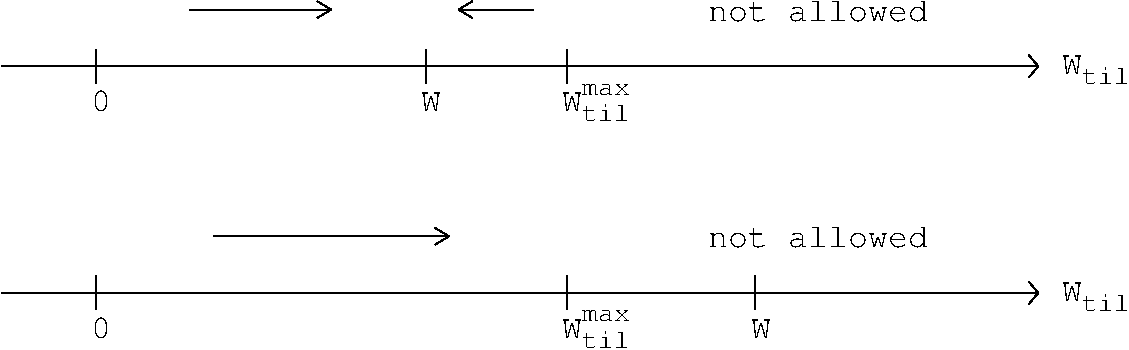
\includegraphics[width=4.5in,keepaspectratio=true]{tillschema}
\bigskip
\caption{The till-stored water amount $\Wtil$ evolves by \eqref{eq:tilldynamics}.  The bounds $0\le \Wtil \le \Wtilmax$ are maintained.  If $\omega W < \Wtilmax$ then $\Wtil$ approaches $\omega W$, from either side.  If $\omega W \ge \Wtilmax$ then $\Wtil$ approaches $\Wtilmax$ from below.}
\label{fig:tillschema}
\end{figure}

Appendix \ref{app:transportstorage} describes an abstract view of the transport-plus-storage model which combines conservation \eqref{eq:conserve} and exchange \eqref{eq:tilldynamics}.  In section \ref{sec:num} we propose a stable numerical scheme for the combination of \eqref{eq:conserve} and \eqref{eq:tilldynamics} which preserves both discrete conservation of $W+\Wtil$ and the bounds $0\le \Wtil \le \Wtilmax$ for the discretized values of $\Wtil$.  


\section{Closures to determine pressure} \label{sec:closures}

At this point we do not know how to compute the water pressure $P$ given the data of the problem, namely $b$, $H$, $m$, $|\bv_b|$, $W$, $\Wtil$, and $Y$.  The (apparent) state variables of the model so far are $W$, $\Wtil$, $Y$, and $P$, but the evolution equations listed so far, namely \eqref{eq:adeqn}, \eqref{eq:hewittcapacity}, and \eqref{eq:tilldynamics}, can only be simplified to three equations in these four unknowns.   A closure is needed.

\subsection*{Closures without cavity evolution}  We consider two simple closures which appear in the literature but which do not use cavity evolution equation \eqref{eq:hewittcapacity} or similar physics.  These simplified closures differ in their physical motivation and the form of their mass conservation equations.  We list them because the resulting simplified conservation equations emerge as steady-state reductions of our more complete theory.  For simplicity we present them without till storage, that is, with $\Wtil=\Wtilmax=0$ in previous equations, and we state only the constant conductivity case ($\alpha=1$ and $\beta=2$ in equation \eqref{eq:flux}).

\renewcommand{\labelenumi}{\textbf{\Roman{enumi}.}}
\begin{enumerate}
\item Setting the pressure equal to the overburden pressure is the simplest closure \citep{Shreve1972}:
\begin{equation}
P = P_o.\label{eq:Pisoverburden}
\end{equation}
This model is sometimes used for ``routing'' subglacial water under ice sheets so as to identify subglacial lake locations \citep{Livingstoneetal2013TCD,Siegertetal2009}.  Straightforward calculations using equations \eqref{eq:conserve}, \eqref{eq:flux}, and \eqref{eq:Pisoverburden} show that the advection-diffusion form \eqref{eq:adeqn} has an ice-geometry-determined velocity,
\begin{equation}
  \frac{\partial W}{\partial t} = - \Div\left(\tilde\bV\, W\right) + \Div\left(\rho_w g k \,W\, \grad W\right) + \frac{m}{\rho_w}   \label{eq:PisoverConservation}
\end{equation}
where
\begin{equation}
\tilde\bV = - \rho_w g k \left[\frac{\rho_i}{\rho_w} \grad h + \left(1-\frac{\rho_i}{\rho_w}\right) \grad b\right].
\end{equation}

Because the approximation $W\ll H$ is usually accepted, so that the hydraulic potential is insensitive to the water layer thickness, i.e.~$\psi = P_o + \rho_w g b$ \citep{Siegertetal2009}, the diffusion term on the right of \eqref{eq:PisoverConservation} is usually not included.  With this common simplification, equation \eqref{eq:PisoverConservation} becomes a pure advection with a velocity $\tilde\bV$ which is independent of $W$.  It therefore possesses characteristic curves \citep{Evans} which are the \emph{a priori} known trajectories of the water flow.  The more complete models we consider in this paper do not have such characteristic curves because they have a flux which depends on the gradient of $W$, the quantity which is being transported.

Equation \eqref{eq:PisoverConservation} as stated, \emph{with} the diffusion term, is well-posed for positive initial and boundary values on $W$ \citep[compare][]{Hewittetal2012}.  Continuum solutions have finite water layer thickness at all times.  By contrast, equation \eqref{eq:PisoverConservation} without the diffusion term, as it usually appears in the literature, will exhibit continuum solutions with infinite concentration at every location where the simplified potential $\psi = P_o + \rho_w g b$ has a minimum.  In fact, applications using the simplified potential tend to only compute the characteristic curves \citep[i.e.~``pathways'',][]{Livingstoneetal2013TCD} and not the evolving field $W$.  Also, because the simplified model is not well-posed, numerical implementations are badly-behaved under grid refinement.

\medskip

\item At an almost opposite extreme in terms of the mathematical form, one might close the model by assuming that the water pressure is locally determined by the amount of water.  \cite{FlowersClarke2002_theory} propose
\begin{equation}
P_{FC}(W) = P_o \left(\frac{W}{W_{\text{crit}}}\right)^{7/2}. \label{eq:PofWFC}
\end{equation}
For Trapridge glacier \cite{FlowersClarke2002_trapridge} use $W_{\text{crit}}=0.1$ m, while Figure \ref{fig:psteady-vb} below illustrates this function with $W_{\text{crit}}=1$ m.  Because of the local relation between water amount and pressure, implementation of a coupled ice flow and subglacial hydrology model is eased because no pressure equation (i.e.~no stress balance within liquid water) needs to be solved \citep{PimentelFlowersSchoof2010,PimentelFlowers2011}.

One obvious concern with form \eqref{eq:PofWFC} is that $P_{FC}(W)$ can be arbitrarily larger than overburden pressure for large amounts of water ($W \gg W_{\text{crit}}$).  Equation \eqref{eq:PofWFC} is not, of course, intended to apply when $W$ is actually large, such as in subglacial lakes.

From \eqref{eq:conserve}, \eqref{eq:flux}, and \eqref{eq:PofWFC} we get the equation:
\begin{equation}
  \frac{\partial W}{\partial t} = \Div\left((\rho_w g k \grad b)\, W\right) + \Div \left(k\,W \grad P_{FC}(W)\right) + \frac{m}{\rho_w}. \label{eq:PofWFCConservation}
\end{equation}
In the flat bedrock case $\grad b=0$ we see that \eqref{eq:PofWFCConservation} is a nonlinear diffusion.  Indeed, \cite{Schoofetal2012} observe that \eqref{eq:PofWFCConservation} generalizes the porous-medium equation $\partial W/\partial t = \grad^2 (W^\gamma)$ \citep{VazquezPME}.  The main idea in such a nonlinear diffusion, and a significant concern when considering applications of \eqref{eq:PofWFC}, is that the direction of the flux is $-\grad W$, while it would seem that the more physical model with $\bq \sim -\grad \psi$ would give flux directions different from $-\grad W$ in many cases, especially in rapidly-evolving hydrologic systems.
\end{enumerate}

\medskip
By constrast with these simple closures, in this paper we apply capacity evolution model \eqref{eq:hewittcapacity} for the distributed system.  However, in steady state conditions our theory recovers a functional relation $P=P(W)$, as shown in Figure \ref{fig:psteady-vb}, but this relation is not a power-law like \eqref{eq:PofWFC}.  Under steady conditions where the ice sliding velocity is zero, our theory also recovers \eqref{eq:Pisoverburden} and \eqref{eq:PisoverConservation}.  Our theory uses advection-diffusion decomposition \eqref{eq:adeqn} and thus in that sense also it extends the ``routing'' model \eqref{eq:PisoverConservation}.  These connections are further exposed in section \ref{sec:steadyverif} below.


\subsection*{Full-cavity closure}  Requiring the subglacial layer to be full of water is a closure for the subglacial pressure $P$, which we adopt in our model:
\begin{equation}
W = Y.\label{eq:strongclosure}
\end{equation}
The consequences of this closure are explored at some length by \cite{Schoofetal2012} and \cite{Hewittetal2012}, who describe the case where cavities are full as the ``normal pressure'' condition (e.g.~equation (4.13) in \cite{Schoofetal2012}).  Their one-dimensional model, which does not include till storage, is the model which comes from taking $\Wtil=\Wtilmax=0$ and $\phi_0=0$ (see below) in our theory.

Equation \eqref{eq:strongclosure} obviously allows us to eliminate either $W$ or $Y$ as a state variable.  We choose to eliminate $Y$ because $W$ is part of the conserved mass $W + \Wtil$.  Using equations \eqref{eq:conserve}, \eqref{eq:hewittcapacity}, and \eqref{eq:strongclosure} we have
\begin{equation}
\mathcal{O}(|\bv_b|,W) - \mathcal{C}(N,W) + \ddt{\Wtil} + \Div\bq = \frac{m}{\rho_w}. \label{eq:elliptic}
\end{equation}

Equation \eqref{eq:elliptic}, a variant of which we will use to determine $P$ (see \eqref{eq:regpressureequation} below) is mostly not new.  In the zero till storage case (set $\Wtilmax=0$ so $\Wtil=0$), equation \eqref{eq:elliptic} is exactly the elliptic pressure equation (2.12) of \cite{Schoofetal2012}.  As in that theory, we could solve \eqref{eq:elliptic}, along with pressure boundary conditions at the lateral edges of the subglacial hydrologic system, for the pressure $P$ given values for the water amount $W$; exactly this is done by \cite{Schoofetal2012}.  They argue, however, that \eqref{eq:elliptic} is not an adequate model of subglacial cavities because it fails to include the possibilities of overpressure, where $W=Y>W_r$ and $P>P_o$, and underpressure, where cavities are partially empty $W<Y$ and at zero pressure $P=0$.  Partially-filled cavities have not been observed except at the margins of glaciers, and not underneath the fast-flowing parts of tidewater glaciers and ice sheets, though of course subglacial hydrology is poorly-observed generally.  The overpressure condition has been observed in ice sheets \citep[for example]{Dasetal08}, but only for durations so short that we cannot foresee application of the current model.

\subsection*{Englacial porosity as a closure regularization}  We agree that \eqref{eq:elliptic} is an inadequate model but we propose an improved model which has a different physical basis.  Englacial systems of cracks, crevasses, and moulins have been observed in glaciers \citep[for example]{Bartholomausetal2008,Harperetal2010}, and these have been included in combined englacial/subglacial hydrology models \citep[among others]{FlowersClarke2002_theory,Bartholomausetal2011,Hewitt2013}.  The englacial system is generally parameterized as having macroporosity $0\le \phi < 1$.  If the englacial system is efficiently-connected to the subglacial water then the amount of englacial water is equivalent to (is determined by and is a linear function of; see below) the subglacial pressure.  Thus, in this hydrologic system, higher or lower subglacial pressure is reflected by higher or lower ``water table'' in the englacial system.  The condition $P\lesssim P_o$ is ``enforced'' on temperate glaciers by the property that water pressure significantly exceeding overburden would cause water to emerge onto the surface of the glacier and stop further increases in pressure.

Appendix \ref{app:barth} shows that an extension of the lumped englacial/subglacial model in \cite{Bartholomausetal2011} to the distributed case gives an equation similar to \eqref{eq:elliptic}, but with the crucial difference that the equation is \emph{parabolic} for the pressure and not \emph{elliptic}.  The time-derivative term is proportional to the englacial porosity $\phi$.  Based on this re-analysis of \cite{Bartholomausetal2011}, we use this parabolic equation in our model with constant notional englacial porosity $\phi=\phi_0$:
\begin{equation}
\frac{\phi_0}{\rho_w g} \ddt{P} = - \Div \bq + \frac{m}{\rho_w} + \mathcal{C}(N,W) - \mathcal{O}(|\bv_b|,W) - \ddt{\Wtil}. \label{eq:regpressureequation}
\end{equation}
If the englacial porosity $\phi_0$ is small, so that there is a nearly impermeable ``cap'' on the subglacial system as would occur under a thick ice sheet, then equation \eqref{eq:regpressureequation} is very stiff and indeed similar, in terms of numerical solution, to an elliptic equation.  However, if $\phi_0$ is relatively large then equation \eqref{eq:regpressureequation} causes local changes in subglacial pressure $P$ to be ``damped'' in the speed and range of their influence on other parts of the connected subglacial hydrologic system.

A more complete model than ours could have spatial variation $\phi(x,y)$ in the englacial porosity so that different parts of the glacier could have different englacial storage capacity.  We will set the porosity constant in the current work, however, both because of an absence of data to determine distributed values for $\phi(x,y)$, and because we use the ``regularizing'' advantage of switching from an elliptic pressure model like the $\Wtilmax=0$ case of \eqref{eq:elliptic} to a parabolic equation \eqref{eq:regpressureequation}.  Indeed, equation \eqref{eq:regpressureequation} is stiff to a degree inversely-proportional to $\phi_0$, in the sense that the range of influence of pressure evolution solutions of the heat-equation-like equation \eqref{eq:regpressureequation} is proportional to $\phi_0$.  The \cite{Schoofetal2012} theory is the infinitely-stiff $\phi_0=0$ extreme case.  The resulting evolution is ``differential-algebraic'' because an elliptic pressure equation is a constraint with no time derivative on the pressure \citep{AscherPetzold}.  In general, stiffer equations are harder to solve numerically, and differential-algebraic equations are hardest.

\cite{Schoofetal2012} show that the time-independent mathematical problem encompassing the $\Wtilmax=0$ case of \eqref{eq:elliptic}, constraints \eqref{eq:bounds}, and appropriate pressure boundary conditions can be written as an elliptic variational inequality \citep{KinderlehrerStampacchia}.  Such mathematical problems in other glaciological free boundary contexts \citep{SchoofStream,JouvetBueler2012}.  This variational inequality problem would be solved at each step of a time-stepping model \citep{Hewitt2013}.  The same difficulty applies to any \emph{implicit} time-stepping scheme using \eqref{eq:regpressureequation}.  Instead, in the current work we give an explicit time-stepping scheme in section \ref{sec:num}, with care to satisfy stability conditions on the time step.

The stiffness of pressure equation \eqref{eq:regpressureequation} follows from the incompressibility of water and the relative non-distensibility (i.e.~hardness) of the ice and bedrock \citep{Clarke2003}.  Our analysis of \eqref{eq:regpressureequation} as a distributed extension of the \cite{Bartholomausetal2011} model shows that this stiffness is moderated if water can flow into englacial porous spaces.  \cite{Clarke2003} addresses stiffness in a physically-different but related way by including in his subglacial water equation a relaxation (damping) parameter  ``$\beta$'' which is based on the small compressibility of water, but which is more than two orders of magnitude larger than the physical value.  \citeapos{Clarke2003} parameter $\beta$ appears in his equation exactly as the englacial porosity $\phi_0$ appears in equation \eqref{eq:regpressureequation}, multiplying the pressure time derivative.
  
Thus we use \eqref{eq:regpressureequation} with constant $\phi_0>0$ both because it is physically-motivated and because it is easier to solve than an elliptic problem.  Because $\bq = - K W \grad \psi$, it is roughly-speaking a diffusion for $P$ in all cases where fine-scale variations in $\psi$ are dominated by fine scale variations in $P$.  It is, in this way of thinking, a diffusion for $P$ coupled to the advection-diffusion equation \eqref{eq:adeqn} for $W$.  Section \ref{sec:num} gives a quantitative analysis of the time-scales related to solving \eqref{eq:regpressureequation}, and the effect of its stiffness on the numerical implementation.

Pressure equation \eqref{eq:regpressureequation} is also a kind of stress balance, a form of conservation of momentum.  There is no obvious way to guarantee that we actually conserve momentum because the enforcement of bounds \eqref{eq:bounds} on $P$ involves large and un-accounted forces \citep{Schoofetal2012}.  However, verifiable conservation of mass is essential in the applications of a subglacial hydrology model.  We carefully consider the numerical conservation of the total water mass $W+\Wtil$ in Section \ref{sec:num}.



\section{A new subglacial hydrology model} \label{sec:newmodel}

\subsection*{Summary of equations and symbols}  The goals of the current work are the selection, implementation, verification, and demonstration of a two-dimensional subglacial hydrology model which is coupled to an existing three-dimensional ice dynamics model.  The new hydrology model must be parallelizable and it must exhibit convergence of solutions under grid refinement.  The remainder of the paper will demonstrate that we have succeeded in these goals.

The major equations for the model are \eqref{eq:adeqn}, \eqref{eq:mohrcoulomb}, \eqref{eq:tilldynamics}, and \eqref{eq:regpressureequation}, collected and re-ordered here, with till effective pressure $\Ntil$ eliminated using equation \eqref{eq:Wtilpressure}:
\begin{empheq}[box=\mybluebox]{align}
\ddt{W} + \ddt{\Wtil} &= - \Div\left(\bV\, W\right) + \Div \left(D \grad W\right) + \frac{m}{\rho_w}, \label{eq:bluebox} \\
\frac{\partial \Wtil}{\partial t} &= \mu \left(\min\left\{\omega W,\Wtilmax\right\} - \Wtil\right), \notag \\
\frac{\phi_0}{\rho_w g} \ddt{P} + \ddt{\Wtil} &= - \Div\left(\bV\, W\right) + \Div \left(D \grad W\right) + \frac{m}{\rho_w} \notag \\
       & \qquad \qquad + c_2 A (P_o - P)^3 W - c_1 |\bv_b| (W_r - W)_+, \notag \\
\tau_c &= c_0 + (\tan \varphi)\, \min\left\{P_o,\, \delta P_o \, 10^{(e_0/C_c) \left(1 - (\Wtil/\Wtilmax)\right)}\right\}. \notag
\end{empheq}
The model also includes bounds on the state variables, namely $0\le W$, $0\le \Wtil \le \Wtilmax$, and $0 \le P \le P_o$.  We also require these associated functions, already defined but collected here:
\begin{align*}
K    &= k W^{\alpha-1} \left|\grad(P+\rho_w g b)\right|^{\beta-2}, \\
\bV  &= - K \grad\left(P + \rho_w g b\right), \\
D    &= \rho_w g K W, \\
\psi &= P + \rho_w g (b + W), \\
P_o  &= \rho_i g H.
\end{align*}
As will be described in section \ref{sec:num}, we have implemented an explicit/implicit adaptive time-stepping numerical scheme for equations \eqref{eq:bluebox} in the Parallel Ice Sheet Model.

\begin{table}[ht]
\caption{Functions used in hydrology model \eqref{eq:bluebox}, including symbol, units, and meaning.}
\begin{tabular}{l|l}
\hline
\emph{state functions} & \begin{tabular}{lll}
        $W$ & m \phantom{llllllllllll\,} & transportable subglacial water layer thickness \\
        $\Wtil$ & m & effective thickness of water stored in till \\
        $P$ & Pa & pressure of transportable water \\
        \end{tabular} \\ \hline
\emph{data functions} &  \begin{tabular}{lll}
        $b$ & m & bedrock elevation \\
        $H$ & m & ice thickness \\
        $m$ & $\text{kg}\,\text{m}^{-2}\,\text{s}^{-1}$ & total melt water input; $=m_{\text{wall}}+m_{\text{drain}}$ \\
        $|\bv_b|$ & $\text{m}\,\text{s}^{-1}$ & ice sliding speed \\
        \end{tabular} \\ \hline
\emph{output} &  \begin{tabular}{lll}
        $\tau_c$ \phantom{l\,} & Pa \phantom{llllllllllll} & till yield stress \\
        \end{tabular} \\ \hline
\end{tabular}
\label{tab:symbols}
\end{table}

\begin{table}[ht]
  \centering
  \caption{Physical constants and model parameters.  Default values are overridden in some experiments.}
  \begin{tabular}{lllp{3.0in}} 
    \textbf{Name} & \textbf{Default Value} & \textbf{Units} & \textbf{Description}\\
\hline
    $A$ & $3.1689\times 10^{-24}$ & $\text{Pa}^{-3}\,\text{s}^{-1}$ & ice softness \citep{EISMINT96} \phantom{$\Big|$} \\
    $\alpha$ & $5/4$ & & power in flux formula  \citep{Schoofetal2012} \\
    $\beta$ & $3/2$ & & power in flux formula  \citep{Schoofetal2012} \\
    $c_0$ & 0 & Pa & till cohesion \citep{Tulaczyketal2000} \\
    $c_1$ & $0.5$ & $\text{m}^{-1}$ & cavitation coefficient \citep{Schoofetal2012} \\
    $c_2$ & $0.04$ & & creep closure coefficient \\
    $C_c$ & 0.12 &  & till compressibility \citep{Tulaczyketal2000} \\
    $\delta$ & 0.01 &  & fraction of overburden pressure \\
    $e_0$ & 0.69 &  & void ratio at $N=N_0$ \citep{Tulaczyketal2000} \\
    $\phi_0$ & $0.01$ & & regularizing englacial porosity \\
    $g$ & $9.81$ & m $\text{s}^{-2}$ & acceleration of gravity \\
    $k$ & $0.01$ & $\text{m}^{2\beta-\alpha} \text{s}^{2\beta-3} \text{kg}^{1-\beta}$ & conductivity coefficient \citep{Schoofetal2012} \\
    $\mu$ & $10^{-6}$ & $\text{s}^{-1}$ & rate constant for evolution of till storage \\
    % \mu = 1/week (about)
    $\rho_i$ & $910$ & $\text{kg}\,\text{m}^{-3}$ & ice density \citep{GreveBlatter2009} \\
    $\rho_w$ & $1000$ & $\text{kg}\,\text{m}^{-3}$ & fresh water density \citep{GreveBlatter2009} \\
    $W_r$ & $0.1$ & $\text{m}$ & roughness scale \citep{Hewittetal2012} \\
    $\Wtilmax$ & $2\phantom{\Big|}$ & $\text{m}$ & max.~water in till \citep{BBssasliding} \\
    $\omega$ & 100 & & transfer ratio for till storage model \\
    \hline
  \end{tabular}
 \label{tab:constants}
\end{table}

Model equations \eqref{eq:bluebox} relate the state functions, data functions, and output function listed in Table \ref{tab:symbols} to the physical constants and model parameters in Table \ref{tab:constants}.  Only the state functions must be provided with initial values, and only they must be saved when stopping and restarting a time-dependent numerical model.  The ``data'' functions are either supplied by true observations or they are provided by other components an ice sheet model (e.g.~the stress balance in an ice dynamics model could provide $\bv_b$).  The output $\tau_c$ is the essential quantity to determine the basal shear stress in the stress balance equations of an ice dynamics model.

The model parameters in Table \ref{tab:constants} are all constant (i.e.~time- and space-independent) in the current paper but they could be allowed to vary spatially if desired.  Although default values must be chosen for the parameters, as is done in Table \ref{tab:constants}, exploration of the parameter space is essential; see section \ref{sec:results}.

\subsection*{Reduction to existing models}  Four reductions (limiting cases) of model \eqref{eq:bluebox} can now be stated precisely:

\renewcommand{\labelenumi}{\textbf{(\roman{enumi})}}
\begin{enumerate}
\item The zero till storage ($\Wtilmax=0$) and zero englacial porosity ($\phi=0$) case of \eqref{eq:bluebox} is the model described by \cite{Schoofetal2012}, recalling that $\bq = - K W \grad \psi$,
\begin{empheq}[box=\mybluebox]{align}
\phantom{dsaf} \frac{\partial W}{\partial t} &= - \Div\left( K W \grad \psi \right) + \frac{m}{\rho_w}, \label{eq:schoofsmodel} \\
0 &= \Div \left( K W \grad \psi \right) + \frac{m}{\rho_w} + c_2 A (P_o - P)^3 W - c_1 |\bv_b| (W_r - W)_+.\phantom{dsaf}  \notag
\end{empheq}
The bounds $W \ge 0$ and $0 \le P \le P_o$ are unchanged.  Model \eqref{eq:bluebox} is a parabolic regularization of \eqref{eq:schoofsmodel} based on a notional connection to porous englacial storage, with a small porosity parameter $\phi_0$, and with coupling to additional till storage.

\item The $P=P_o$ limit of \eqref{eq:bluebox}, in which physical processes for the evolution of pressure are ignored and the pressure reverts to overburden, is the standard model for ``routing'' water to subglacial lakes under cold ice sheets \citep{Livingstoneetal2013TCD,Siegertetal2009}.  Assuming again that till storage is removed ($\Wtilmax=0$) then the model has only $W$ as a state variable.  The pressure is not an unknown, the parameterization of cavity evolution is inactive, and the pressure evolution equation is not needed.  There is now less stiffness because the model is an advection using a mostly-geometrically-determined velocity.    The single evolution equation is
\begin{empheq}[box=\mybluebox]{align}
\phantom{ldsfj} \frac{\partial W}{\partial t} &= - \Div\left(\bV\, W\right) + \Div \left(D \grad W\right) + \frac{m}{\rho_w}. \phantom{ldsfj} \label{eq:lakesmodel}
\end{empheq}
along with the bound $W \ge 0$ and additional definitions $\psi = P_o + \rho_w g (b + W)$, $K = k W^{\alpha-1} \left|\grad \psi\right|^{\beta-2}$, $\bV = - K \grad \left(P_o + \rho_w g b\right)$, and $D = \rho_w g K W$.  As noted in section \ref{sec:closures}, the $\alpha=1$ and $\beta=2$ case of this model routes water with a velocity which is determined entirely by ice and bedrock geometry.  Because of the way we have including $W$ into the hydraulic potential, so that large $W$ implies some diffusion, model \eqref{eq:lakesmodel} is well-posed and has continuous solutions and it therefore represents a modest improvement to these ``routing'' models.

\item Again setting till storage to zero ($\Wtilmax=0$), the non-distributed ``lumped'' form of \eqref{eq:bluebox}, in which $\Div \bq = (q_{out} - q_{in})/L$ where $L$ is the length of the glacier and $q_{out},q_{in}$ are given by observations, is the porous glacier model of \cite{Bartholomausetal2011}.  The correspondence is further explained in Appendix \ref{app:barth}, with an emphasis on the pressure equation which applies in that lumped model.

\item If the lateral transport model is absent then exchange equation \eqref{eq:tilldynamics} is not needed.  Now water input $m$ goes directly into till storage.  The undrained plastic bed (UPB) of \cite{Tulaczyketal2000b} is such a model; it arises as the $W=0,\bq=0,\phi=0,c_1=0,c_2=0$ reduction of \eqref{eq:bluebox} in which a constant reference effective pressure $N_0$ is used (instead of one that scales with overburden, e.g.~as ``$N_0=\delta P_o$'' in this paper):
\begin{empheq}[box=\mybluebox]{align}
\phantom{foo} \ddt{\Wtil} &= \frac{m}{\rho_w}, \label{eq:upbbox} \\
\tau_c &= c_0 + (\tan \varphi)\, N_0\, 10^{(e_0/C_c) \left(1 - (\Wtil/\Wtilmax)\right)}, \phantom{mm} \notag
\end{empheq}
UPB depends on friction-heating feedback to keep $\Wtil$ bounded, which does not work in a membrane-stress-including theory, in which friction heating is a non-local effect of local changes in till strength.  \cite{BBssasliding} therefore enforce $\Wtil \le \Wtilmax$ by non-conservatively removing water that would raise $\Wtil$ above the bound; this is a minimal ``drained'' version of the UPB model.  The model implemented in PISM has additional diffusion and a linearization of the second of the above equations (so that $\tau_c$ is a linear function of $\Wtil$) \citep{BBssasliding}.  The current paper seeks to improve PISM by implemention of a model which has transport and is mass-conservative.
\end{enumerate}

The above list is not intended to suggest that all subglacial hydrology is subsumed in our model.  For example, the subglacial hydrology model of \cite{JohnsonFastook} could be considered as a variation on the idea \textbf{(ii)} but, specifically because it has a velocity that depends on second derivatives of the surface elevation, it cannot be considered a reduction of our model.  The \cite{FlowersClarke2002_theory} model is also not a reduction, although a significant connection is explained in the next section on steady states.

Most significantly, those models that include conduits \citep[among others]{Hewittetal2012,PimentelFlowers2011,Schoofmeltsupply} are not reductions of our model.  Conduit evolution is numerically-straightforward to implement in one-dimensional hydrology models \citep{Hewittetal2012,PimentelFlowers2011,vanderWeletal2013} but when extended to two-horizontal dimensions all existing models \citep{Hewitt2013,Schoofmeltsupply} become ``lattice'' models without a known continuum limit.  Such modeling choices are incompatible with general-purpose continuum-approximating models like PISM where users determine grid spacing at run-time.  The hydrology submodel in PISM is only acceptable if it exhibits convergence under grid refinement.


\section{Steady states}  \label{sec:steadyverif}

\subsection*{Processes become decoupled in steady state}  The steady states of mathematical model \eqref{eq:bluebox} are worth considering for at least three reasons: (\emph{i}) the physical subglacial system is close to steady state much of the time, (\emph{ii}) we can more clearly identify vaious contributions to the water flux in steady state (equation \eqref{eq:qabstract} below), and (\emph{iii}) we can find an exact solution in two spatial variables.  We will also see that in steady state there is a function which relates the water pressure $P$ directly (locally) to the water amount $W$, though no such function exists in the time-dependent theory.

In this section we address only the $\alpha=1$ and $\beta=2$ case but the major conclusions apply generally.  Furthermore we remove till storage from the model ($\Wtilmax=0$).  The steady form of model \eqref{eq:bluebox}, with these simplifications, can be written in terms of $\bV,\bq,W,P$:
\begin{align}
\bV &= - k \grad \left(P + \rho_w g b\right), \label{eq:Vsteady} \\
\bq &= \bV W - \rho_w g k W \grad W, \label{eq:qsteady} \\
0 &= - \Div \bq + \frac{m}{\rho_w}, \label{eq:masscontsteady} \\
0 &= c_2 A (P_o - P)^3 W - c_1 |\bv_b| (W_r - W)_+. \label{eq:openclosesteady}
\end{align}
Note that we also have bounds $W\ge 0$ and $0 \le P \le P_o$.

Relative to the time-dependent form \eqref{eq:bluebox}, processes have become decoupled in the steady state equations \eqref{eq:Vsteady}--\eqref{eq:openclosesteady}.  There are separate balances between the divergence of the flux and the water input on the one hand (equation \eqref{eq:masscontsteady}), and the opening and closing processes on the other hand (equation \eqref{eq:openclosesteady}).  Steady state equations \eqref{eq:Vsteady}--\eqref{eq:openclosesteady} are also stated by \cite{Schoofetal2012} model, where the decoupling is also noted.  Specifically, in the one-dimensional case the above equations reduce to (5.8) and (5.10) from \cite{Schoofetal2012}.

\subsection*{Functional relationship for pressure in steady state}  Equation \eqref{eq:openclosesteady} allows us to write the pressure $P=P(W)$ in steady state as a continuous function of the water amount $W$.  (This fundamental fact was already pointed out in considering the steady states of equation \eqref{eq:hewittcapacity}.)  Steady state is only possible if condition \eqref{eq:steadyOCbound} holds, but here with $W$ for $Y$:
\begin{equation}
c_1 |\bv_b| (W_r - W)_+ \le c_2 A P_o^3 W \qquad \text{ in steady state}. \label{eq:steadyboundfirst}
\end{equation}
In this and later formulas define the following scaled basal sliding speed which has units of pressure:
\begin{equation}
s_b =  \left(\frac{c_1 |\bv_b|}{c_2 A}\right)^{1/3}.  \label{eq:definesb}
\end{equation}
One may think of $s_b$ as a scale for the pressure drop associated to cavitation in steady state.  Then \eqref{eq:steadyboundfirst} is equivalent to
\begin{equation}
W \ge W_c := \frac{s_b^3}{s_b^3 + P_o^3} W_r  \qquad \text{ in steady state}. \label{eq:steadyboundsecond}
\end{equation}
This condition says that the water amount is above a critical level that depends on the sliding and the overburden pressure.  If the pressure effect sliding is large ($s_b \gg P_o$) then $W_c\approx W_r$.

If \eqref{eq:steadyboundfirst} or \eqref{eq:steadyboundsecond} holds then
\begin{equation}
P(W) = P_o - s_b \left(\frac{(W_r - W)_+}{W}\right)^{1/3} \qquad \text{ in steady state}.  \label{eq:PofWsteady}
\end{equation}
Note that in \eqref{eq:PofWsteady} we have $P(W_c)=0$.  Underpressure ($P=0$) with subcritical water amount ($W<W_c$) does not occur \emph{in steady state} though it can occur in nonsteady conditions.  Formula \eqref{eq:PofWsteady} may apply even if $W\ge W_r$, in which case the water pressure takes the overburden value $P = P_o$.  However, if $P_o=0$ then \eqref{eq:steadyboundfirst} implies that either $W\ge W_r$ or $|\bv_b|=0$.  This describes the values of $W$ and $|\bv_b|$ at ice margins where $H\to 0$ and therefore $P_o\to 0$.  These are all restrictions that apply when $W=Y$, that is, when the cavities are full, whereas partially-filled cavities can occur in the \cite{Schoofetal2012} theory.

\newcommand{\upto}{ \!\!\nearrow\! }
\newcommand{\downto}{ \!\searrow\! }
Figure \ref{fig:psteady-vb} shows the function $P(W)$ from \eqref{eq:PofWsteady} for several cases of sliding speed $|\bv_b|$.  Figure \ref{fig:psteady-Po} shows $P(W)$ for several cases of overburden pressure $P_o$.  We see that as the water amount reaches the roughness scale ($W\upto W_r$) the pressure rises rapidly to overburden ($P(W) \upto P_o$).  At the other extreme, we see that $P(W) \downto 0$ if $W \downto W_c$.  The curves $P(W)$ in Figures \ref{fig:psteady-vb} and \ref{fig:psteady-Po}, which describe steady state, do not include the interval $0\le W < W_c$ because such underpressure conditions are not achievable in steady state.

\begin{figure}[ht]
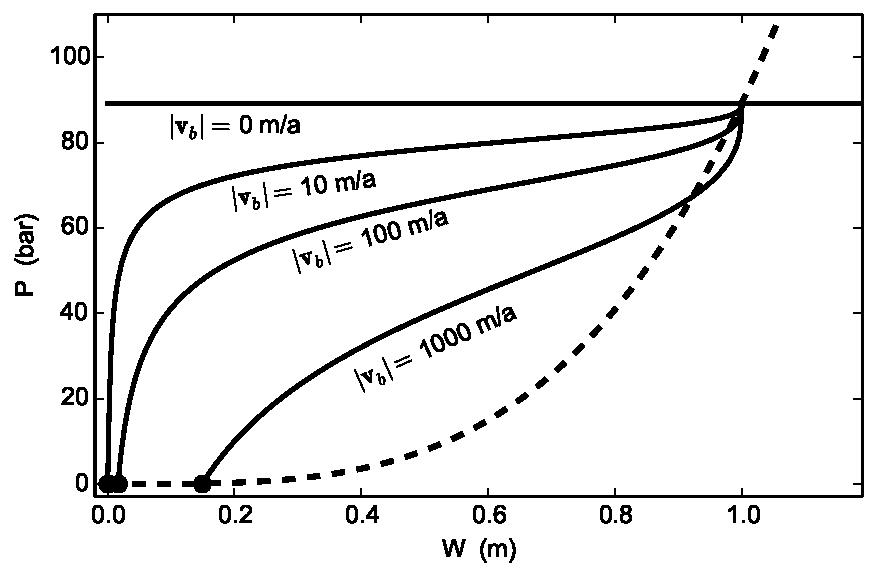
\includegraphics[width=3.5in,keepaspectratio=true]{psteady-vb}
\medskip
\caption{The steady state function $P(W)$ defined by equation \eqref{eq:PofWsteady} depends on the sliding speed.  Four cases with $W_r=1$ m are shown in color using a fixed uniform ice thickness of $H=1000$ m: $|\bv_b|=0$ m/a (blue), $10$ m/a (green), $100$ m/a (red), and $1000$ m/a (cyan).  The values of $W_c$ for these cases are indicated by black dots at $P=0$.  Relation \eqref{eq:PofWFC} (dashed black) is shown with $W_{\text{crit}}=1$ m for comparison.}
\label{fig:psteady-vb}
\end{figure}

\begin{figure}[ht]
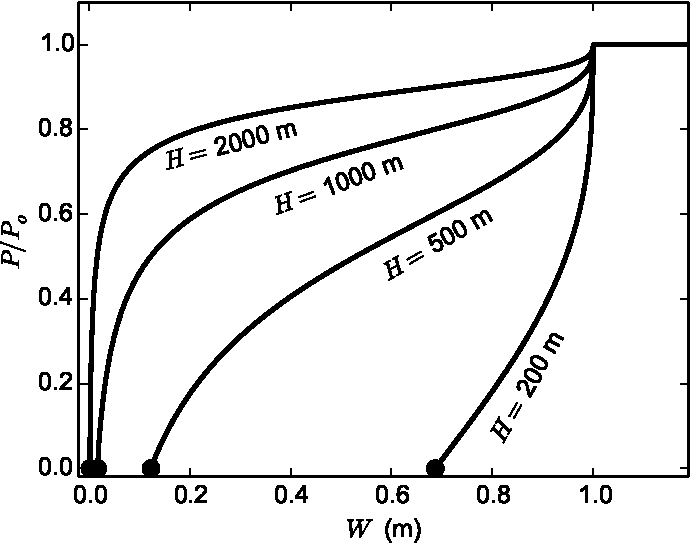
\includegraphics[width=3.5in,keepaspectratio=true]{psteady-Po}
\medskip
\caption{Function $P(W)$ defined by \eqref{eq:PofWsteady} also depends on overburden pressure $P_o=\rho_i g H$.  We fix $|\bv_b|=100$ m/a and $W_r=1$ m and consider four cases of uniform thickness $H=$ $2000$ m (blue), $1000$ m (green), $500$ m (red), and $200$ m (cyan).}
\label{fig:psteady-Po}
\end{figure}

Recall that \cite{FlowersClarke2002_theory} propose function $P_{FC}(W)$ (equation \eqref{eq:PofWFC}) for both steady and nonsteady circumstances.  Both functions $P(W)$ in \eqref{eq:PofWsteady} and $P_{FC}(W)$ are increasing and both relate the water pressure to the overburden pressure $P_o$.  However, while in \eqref{eq:PofWsteady} the relation to $P_o$ is additive, in \eqref{eq:PofWFC} it is a multiplicative scaling.  The power law form \eqref{eq:PofWFC} is not justified by the physical reasoning which led to equation \eqref{eq:PofWsteady}, even in steady state.   It would appear that any functional relationship $P(W)$ should also depend on the sliding velocity, as it does here, if cavitation is to influence the water pressure.  Of course the $W>W_{\text{crit}}$ case gives $P_{FC}(W) > P_o$ in \eqref{eq:PofWFC}, a problematic condition already noted by \cite{Schoofetal2012}, but this condition does not arise in \eqref{eq:PofWsteady}.  In conclusion, an important contrast between the \cite{FlowersClarke2002_theory} theory and the current paper is that we will not assume a relationship $P=P(W)$ in nonsteady conditions, even though such a relation does emerge from our theory in steady state.

\subsection*{Water velocity in steady state}  We now consider how the steady state water velocity $\bV$ depends on other quantities.  Equation \eqref{eq:PofWsteady} defines $P=P(W,P_o,s_b)$ while $\bV$ depends on $\grad P$.  Thus we need derivatives of $P$.  In steady state we have
\begin{equation}
\frac{\partial P}{\partial W} =
    \begin{cases}
      \text{undefined}, & W \le W_c, \\
      \frac{1}{3} s_b W_r W^{-4/3} (W_r - W)^{-2/3}, & W_c < W < W_r, \\
      \text{undefined}, & W = W_r, \\
      0, & W > W_r.
    \end{cases}  \label{eq:dPdWsteady}
\end{equation}
Note that the condition $W_c < W < W_r$ is identical to the normal pressure condition $0 < P < P_o$ in steady state.  Formula \eqref{eq:dPdWsteady} and Figures \ref{fig:psteady-vb} and \ref{fig:psteady-Po} agree that $\partial P / \partial W \to \infty$ as $W \upto W_r$.  

Equations \eqref{eq:Vsteady}, \eqref{eq:PofWsteady}, and \eqref{eq:dPdWsteady} now yield a formula for the velocity in steady state which applies in the normal pressure cases:
\begin{align}
\bV &= - k \grad P - \rho_w g k \grad b = - k \left[\frac{\partial P}{\partial P_o} \grad P_o + \frac{\partial P}{\partial s_b} \grad s_b + \frac{\partial P}{\partial W} \grad W\right] - \rho_w g k \grad b  \notag \\
    &= - k \left[\grad \left(P_o + \rho_w g b\right) - \left(\frac{W_r - W}{W}\right)^{1/3} \grad s_b + \frac{s_b W_r}{3 W^{4/3} (W_r - W)^{2/3}} \grad W\right]. \label{eq:Vsteadyexpand}
\end{align}
Formula \eqref{eq:Vsteadyexpand} helps us understand the steady state meaning of the advective flux ``$\bV W$'' in $\bq=\bV W - D \grad W$.  The direction of water velocity $\bV$ is determined by a combination of a geometric direction ($-\grad \left(P_o + \rho_w g b\right)$), a direction derived from spatial variations in the sliding speed ($\grad s_b$), and a diffusive direction ($-\grad W$).  Therefore a fraction of $\bV W$ is diffusive in steady state,\footnote{To our knowledge, the identification of the diffusiveness of this steady velocity is new to this paper.} in addition to the \emph{a priori} diffusive flux $- D \grad W$.

Let $\psi_o = P_o + \rho_w g b$ for simplicity.  We see that in steady state we can write the flux as a linear combination of gradients,
\begin{equation}
\bq = \bV W - D \grad W = - A_1 \grad \psi_o + A_2 \grad s_b - A_3 \grad W,  \label{eq:qabstract}
\end{equation}
with coefficients
\begin{equation}
A_1 = k W, \quad
A_2 = k \left(W_r - W\right)^{1/3} W^{2/3}, \quad
A_3 = \frac{k s_b W_r}{3 (W_r - W)^{2/3}}\, W^{-1/3} + \rho_w g k W.
\end{equation}
The first two coefficients $A_{1,2}$ go to zero as $W\to 0$.  However, $A_3$ remains large when $W\to 0$, even if $k$ is small, as long as sliding is occurring ($s_b > 0$).  Thus for low water amount and sustained sliding we should think of the water as diffusing in the layer; the apparently advective term ``$\bV W$'' is acting diffusively.  When the water thickness is much greater, specifically if it approximates the roughness scale ($W\approx W_r$), then $A_1$ is more significant, $A_2$ is again small, and $A_3$ may be significant in sliding cases ($s_b>0$).

Thinking more generally, it would be no surprise that when the ice thickness, bed elevation, sliding velocity, or water thickness fields is highly-variable in space then we can expect larger speeds $|\bV|$ in steady state.  Considering the various gradients in it, formula \eqref{eq:qabstract} reflects this general intuition.  Because the magnitude of the velocity determines the CFL time step restriction \citep{MortonMayers} associated to numerically solving the mass conservation equation, large variations in these spatial fields will also generally reduce the time steps taken by a numerical model.

\subsection*{The radial steady-state equations}  The above steady equations are the basis on which we now build a nearly-exact solution for $W$ and $P$ in the map-plane.  This solution, which is useful for verifying time-stepping or time-independent numerical schemes, will depend on the numerical solution of a scalar first-order ODE initial value problem, something we can do with high accuracy.  Exact solutions in one horizontal dimension (waves) also appear in \cite{Schoofetal2012}.

Consider steady state equations \eqref{eq:Vsteady}--\eqref{eq:masscontsteady}, and assume all quantities only depend on the radial coordinate $r = \sqrt{x^2+y^2}$.  One may eliminate $\bV$.  In the flat bed case the resulting pair of equations is
\begin{align}
q &= - k W\, \left(\frac{dP}{dr} + \rho_w g \frac{dW}{dr}\right), \label{eq:rsflux} \\
\frac{1}{r}\frac{d}{dr}\left(r\,q\right) &= \frac{m}{\rho_w}. \label{eq:rsconserve}
\end{align}

In the case of constant water input where $m = m_0 > 0$, which we assume for the exact solution, we can integrate \eqref{eq:rsconserve} from $0$ to $r$ and use symmetry ($q(0)=0$) to get
\begin{equation}
q(r) = \frac{m_0}{2\rho_w} \, r. \label{eq:qradial}
\end{equation}
On the other hand, equation \eqref{eq:PofWsteady} gives $P$ as a function of $W$ in steady state; here equation \eqref{eq:openclosesteady} has played the key role.  Suppose $h(r)$ is given so that $P_o(r)$ is also determined.  Assume that the scaled sliding speed $s_b(r)$ has a bounded derivative and that the solution $W(r)$ satisfies the normal pressure conditions $W_c < W < W_r$; both of these properties must be verified later for the constructed solution.  Now, by combining \eqref{eq:PofWsteady}, \eqref{eq:dPdWsteady}, \eqref{eq:rsflux}, and \eqref{eq:qradial} we can eliminate $q$ and $P$ to find
\begin{equation}
\omega_0\, r = - W\, \left(\frac{dP_o}{dr} - \frac{ds_b}{dr} \left(\frac{W_r - W}{W}\right)^{1/3} + \left(\frac{s_b W_r}{3 W^{4/3} (W_r - W)^{2/3}} + \rho_w g\right) \frac{dW}{dr}\right)  \label{eq:ODEfirst}
\end{equation}
where $\omega_0 = m_0 / (2 \rho_w k)$.

Equation \eqref{eq:ODEfirst} is a first-order ordinary differential equation (ODE) for $W(r)$.  To put it in the standard form expected by a numerical ODE solver we solve it for $dW/dr$:
\begin{equation}
\frac{dW}{dr} = \frac{\frac{ds_b}{dr} W (W_r - W) - \Big[\omega_0\, r W^{-1} + \frac{dP_o}{dr}\Big] W^{4/3} \left(W_r - W\right)^{2/3}}{\frac{1}{3} s_b W_r + \rho_w g W^{4/3} (W_r - W)^{2/3}}.
\label{eq:WradialODE}
\end{equation}
Equation \eqref{eq:WradialODE} has a constant solution $W(r)=W_r$.

\subsection*{Generating a nontrivial exact solution}  To generate a nontrivial exact solution, however, we will have a positive thickness of ice at the margin so that $P_o(L^-)>0$; Figure \ref{fig:Pexact} shows this small cliff at the margin.  We also assume that at the margin there is some sliding so that $s_b(L^-)>0$, and we require that $s_b(L^-) W_r > P_o(L^-)^3 Y_0$.  At the ice margin $r=L$ we have water pressure $P=0$ so $W(L)=W_c(L^-)$ is the boundary (initial) condition for the ODE.  The initial condition at $r=L$ also satisfies $W(L) < W_r$.  Then we integrate \eqref{eq:WradialODE} from $r=L$ to $r=0$.  The central water thickness value $W(0)$ is determined as part of the solution.

It is useful to have an ice cap geometry in which the surface gradient formula is simple so that $dP_o/dr$ in \eqref{eq:WradialODE} is also simple.  The plug flow, flat bed surface elevation solution of \cite{Bodvardsson} has this property.  Extending to the radial case, equations (23) and (24) of \citep{Bodvardsson} give ice thickness
\begin{equation}
H(r) = H_0 \left(1 - \frac{r^2}{R_0^2} \right) \label{eq:choosebodvardssonh}
\end{equation}
where $H(0)=H_0$ is the height of the center of the ice cap.  It follows that $dP_o/dr = - C r$ where $C=2\rho_i g h_0 R_0^{-2}$.  We choose $L=0.9 R_0$ and we note that $H(L)=0.19 h_0$ in \eqref{eq:choosebodvardssonh}.

The sliding speed could be determined by a model for stresses at the ice base and within the ice \citep{GreveBlatter2009}, but a coupled ice and water dynamics solution is too advanced for initial model verification.  Instead we choose a well-behaved sliding speed function which has no sliding near the ice cap center, and which increases in the radial direction:
\begin{equation}
|\bv_b|(r) = \begin{cases} 0, & 0 \le r \le R_1, \\
                           v_0  \left(\frac{r-R_1}{L-R_1}\right)^5, & R_1 < r \le L.
             \end{cases}  \label{eq:choosevb}
\end{equation}
It follows from \eqref{eq:definesb} and \eqref{eq:choosevb} that $ds_b/dr$ in \eqref{eq:WradialODE} is bounded and continuous on $0\le r \le L$.

Now we solve ODE \eqref{eq:WradialODE} with initial condition $W(L)=W_c(L)$ and the specific values in Table \ref{tab:verifconstants}.  We use adaptive numerical ODE solvers, both a Runge-Kutta 4(5) Dormand-Prince method and a variable-order stiff solver, with relative tolerance $10^{-12}$ and absolute tolerance $10^{-9}$, and with essentially identical results.  Modest stiffness \citep{AscherPetzold} of ODE \eqref{eq:WradialODE} is observed at $r\approx R_1$.  The result $W(r)$ is shown in Figure \ref{fig:Wexact}.

Because equations \eqref{eq:choosebodvardssonh} and \eqref{eq:choosevb} imply a pressure functional relation $P=P(W,r)$ from \eqref{eq:PofWsteady}, we can also show in Figure \ref{fig:Wexact} the regions of the $r,W$ plane which correspond to overpressure, normal pressure, and underpressure.  We see that $W(r)$ is in the normal pressure region as $r$ decreases from $r=L$ to $r=R_1$.  At $r=R_1$ the function $W(r)$ switches into the overpressure case because there is no sliding.  Figure \ref{fig:Pexact} shows the corresponding pressure solution $P(r)=P(W(r))$ from \eqref{eq:PofWsteady}.

\begin{table}[ht]
  \centering
  \caption{Constants used in constructing the exact solution.}
  \begin{tabular}{lllp{3.0in}}
    \textbf{Name} & \textbf{Value} & \textbf{Units} & \textbf{Description}\\
\hline
    $\alpha$ & $1$ & & power in flux \\
    $\beta$  & $2$ & & power in flux \\
    $H_0$ & $500$ & m & ice cap center thickness \\
    $k$   & $0.01/(\rho_w g)$ & $\text{m}^3\,\text{s}\,\text{kg}^{-1}$ & hydraulic conductivity; FIXME: 4 orders of magnitude smaller than in \cite{Hewittetal2012} \\
    $L$   & $22.5$& km & $=0.9 R_0$; actual ice cap margin \\
    $m_0$ & $0.2\rho_w$ & $\text{kg}\,\text{m}^{-2}\,\text{a}^{-1}$ & constant water input rate; $= 20 \,\text{cm}\,\text{a}^{-1}$ \\
    $R_0$ & $25$  & km & ideal ice cap radius \\
    $R_1$ & $5$   & km & radial location $r=R_1$ of onset of sliding \\
    $v_0$ & $100$ & $\text{m}\,\text{a}^{-1}$ & sliding speed scale \\
    $W_r$ & $1$ & m & roughness scale \\
    $\Wtilmax$ & 0 & m & (thus no water in till) \\
    \hline
  \end{tabular}
 \label{tab:verifconstants}
\end{table}

\begin{figure}[ht]
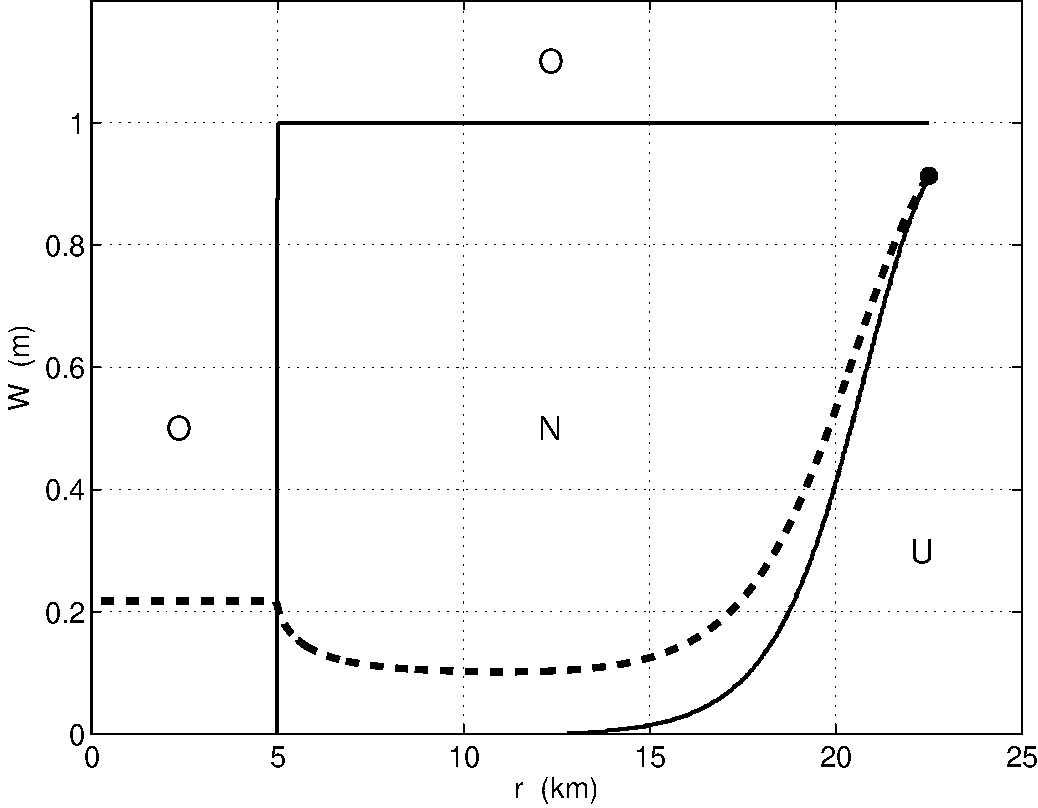
\includegraphics[width=3.5in,keepaspectratio=true]{exact-W-plot-onu}
\caption{An exact radial, steady solution for water thickness $W(r)$ (dashed).  In $r$-versus-$W$ space the overpressure (O), normal pressure (N), and underpressure (U) regions are determined by ice geometry and sliding velocity (solid curves; see text).}
\label{fig:Wexact}
\end{figure}

The reason for stiffness near $R_1$ is that as the sliding goes to zero the cavitation also goes to zero.  Because creep closure balances cavitation in steady state, effective pressure also goes to zero ($P\to P_o$).  The remaining active mechanisms in the model are the variable overburden pressure and the rate of water input.  They must exactly balance.  In fact, in this case \eqref{eq:WradialODE} reduces to the much simpler form
\begin{equation}
\frac{dW}{dr} = - \frac{\varphi_o r W^{-1} + \frac{dP_o}{dr}}{\rho_w g}. \label{eq:WradialODEnoslide}
\end{equation}
Though we have not derived it this way, Equation \eqref{eq:WradialODEnoslide} is the steady radial form of the mass conservation equation under the ``$P=P_o$'' closure, namely equation \eqref{eq:PisoverConservation}.

In equation \eqref{eq:WradialODEnoslide} we see that $dW/dr=0$ if $W$ satisfies $W = - \varphi_0 r / (dP_o/dr)$.  In our case with geometry \eqref{eq:choosebodvardssonh} this reduces to a constant value $W=\tilde W= 0.21764$ m because $\Phi_0$ is constant and $dP_o/dr$ is linear in $r$.  Both numerical ODE solvers used here confirm that $W(r)$ is asymptotic to this constant value $\tilde W$ as $r\to 0$, and that $W(r)\approx \tilde W$ within about 1\% on all of $0\le r \le R_1$.  This is seen in Figure \ref{fig:Wexact}.

\begin{figure}[ht]
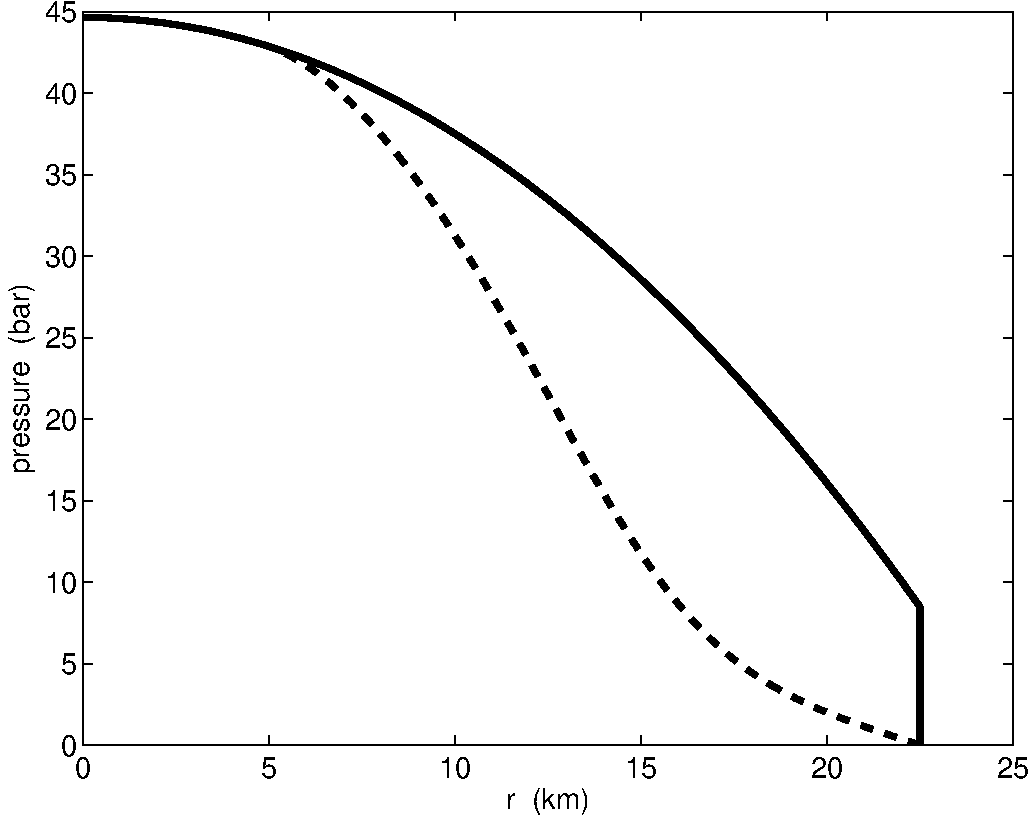
\includegraphics[width=3.5in,keepaspectratio=true]{exact-P-plot}
\caption{An exact radial, steady solution pressure $P(r)$ (dashed) and overburden pressure $P_o$ (solid).}
\label{fig:Pexact}
\end{figure}
%FIXME: consider showing this figure with different values for $v_0$


\section{Numerical schemes}  \label{sec:num}

\subsection*{Time-scales for the discrete mass conservation equation}  Mass conservation equation \eqref{eq:adeqn}, which is part of the combined mathematical model \eqref{eq:bluebox}, will be discretized by a mostly-explicit, conservative finite difference method.   A centered, second-order scheme will be applied to the diffusion part.  A pair of schemes for the advection part will be compared, namely first-order upwinding and a higher-order flux-limited upwind-biased method.

We first consider stable time steps.  Stability for either advection scheme occurs with a time step $\Delta t \le \Delta t_{\text{CFL}}$ where
\begin{equation}
\Delta t_{\text{CFL}} \left(\frac{\max |u|}{\Delta x} + \frac{\max |v|}{\Delta y}\right) = \frac{1}{2}. \label{eq:dtCFL}
\end{equation}
Because of the additional diffusion process, for stability the time step should also satisfy $\Delta t \le \Delta t_{W}$  where \citep{MortonMayers}
\begin{equation}
\Delta t_W\, 2 \max D \left(\frac{1}{\Delta x^2} + \frac{1}{\Delta y^2}\right) = \frac{1}{2}. \label{eq:dtDIFFW}
\end{equation}
The condition $\Delta t \le \min\{\Delta t_{\text{CFL}}, \Delta t_W\}$ is sufficient for stability and convergence of the overall scheme for \eqref{eq:adeqn}.  Appendix \ref{app:positivestable} shows this for the first-order upwind scheme, while standard theory suggests the same conclusion for the higher-order flux-limited advection scheme \citep{HundsdorferVerwer2010}.

We can understand the scale of these restrictions better by considering an example using the parameter values in Table \ref{tab:constants}.  We ran the model on a $\Delta x = \Delta y = 250$ m grid to approximate steady state for the subglacial hydrology of \Nbreen, using observed ice and bedrock geometry, a hypothesized water input distribution with average value about 1 m $\text{a}^{-1}$, and a glacier-wide constant sliding rate of $50$ m $\text{a}^{-1}$.  The result is that the maximum computed water speed $|\bV|$ is about $0.2$ m $\text{s}^{-1}$ so the advective restriction \eqref{eq:dtCFL} is $\Delta t_{\text{CFL}} \approx 300\,\text{s} \approx 10^{-5}\,\text{a}$.  Computed diffusivity $D = \rho_w g K W$ has a maximum value that varies in time, $0.1 \le \max D \le 5 \,\text{m}^2\,\text{s}^{-1}$.  For example, diffusive restriction \eqref{eq:dtDIFFW} with representative value $\max D=1\,\text{m}^2\,\text{s}^{-1}$ is $\Delta t_W \approx 8000\,\text{s} \approx 2.5 \times 10^{-4}\,\text{a}$.  Thus in this simulation $\Delta t_W \approx 25 \Delta t_{CFL}$.

This example suggests that, unless both the global peak velocity is unusually slow, and deep subglacial lakes develop so that $D$ is large, the diffusive time scale is significantly longer than the CFL time scale for a $250$ m grid.  However, the scaling $\Delta t_W = O(\Delta x^2)$ versus $\Delta t_{CFL} = O(\Delta x^1)$ makes it clear that under sufficient spatial grid refinement $\Delta t_W$ is the controlling restriction.  We will see below, however, that the time step restriction associated to an explicit time-stepping method for the pressure equation is typically shorter than either of $\Delta t_W,\Delta t_{CFL}$, and it scales as $O(\Delta x^2)$ like $\Delta t_W$.  By contrast, if implicit time-stepping is used for the pressure equation \citep{Hewittetal2012,Schoofetal2012} then the time scales $\Delta t_W, \Delta t_{CFL}$ addressed here are the only restrictions.  The time step restriction $\Delta t_W$ could be removed by implicit steps for the mass-conservation equation, though this requires another variational inequality formulation because of the lower bound $W\ge 0$ \citep[compare][]{JouvetBueler2012}.  Our observation that $\Delta t_{CFL} \ll \Delta t_W$ suggests that implicit time-stepping for the mass-conservation equation would not be beneficial.

\begin{figure}[ht]
\centering
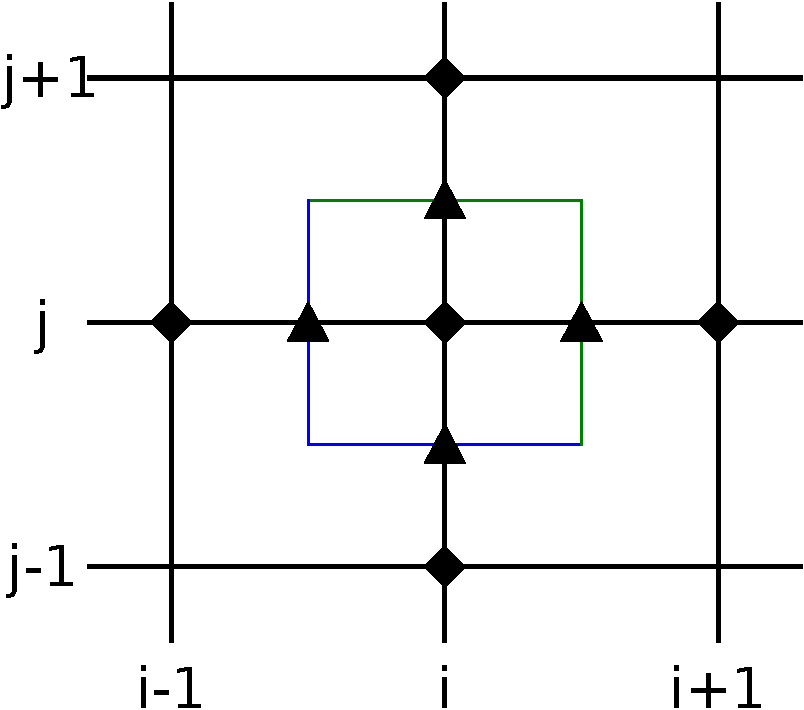
\includegraphics[width=2.5in,keepaspectratio=true]{diffstencil}
\bigskip
\caption{Numerical schemes \eqref{eq:Wfd} and \eqref{eq:Pfd} use a grid-point-centered cell.  Velocities, diffusivities, and fluxes are evaluated at staggered grid locations (triangles at centers of cell edges denoted $e,w,n,s$).  State functions $W,P$ are located at regular grid points (diamonds).}
\label{fig:stencil}
\end{figure}

\subsection*{Discretization of the mass conservation equation}  To set notation, suppose the rectangular computational domain has $M_x \times M_y$ gridpoints $(x_i,y_j)$ with uniform spacing $\Delta x,\Delta y$.  Let $\Wlij \approx W(t_l,x_i,y_j)$, $(\Wtil)_{ij}^l \approx \Wtil(t_l,x_i,y_j)$, and $\Plij \approx P(t_l,x_i,y_j)$ denote the numerical approximations.

We will compute velocity components and flux components at the staggered (cell-face-centered) points shown in Figure \ref{fig:stencil} using centered finite difference approximations of equations \eqref{eq:vexpression} and \eqref{eq:qexpression}.  We use ``compass'' indices such as $u_e = u_{i+1/2,j}$ for the ``east'' staggered component.  Similarly we use compass indices for staggered grid values of the water layer thickness, computed by averaging regular grid values:
\begin{equation}
W_e = (W_{i,j}^l + W_{i+1,j}^l)/2, \qquad W_n = (W_{i,j}^l + W_{i,j+1}^l)/2. \label{eq:stagW}
\end{equation}
We can compute the ``west'' and ``south'' values by shifting indices: $W_w = W_e\big|_{(i-1,j)}$ and $W_s = W_n\big|_{(i,j-1)}$.  Thus there are only two distinct staggered grid values (e.g.~east and north) to compute per regular grid location $(x_i,y_j)$.
The nonlinear effective conductivity $K$ from \eqref{eq:Kdefine} is also needed at staggered locations.  As a notational convenience define $R=P+\rho_w g b$ and define these staggered-grid values \citep[compare][]{Mahaffy}:
\begin{align*}
\Pi_e &= \left|\frac{R_{i+1,j}-R_{i,j}}{\Delta x}\right|^2 + \left|\frac{R_{i+1,j+1}+R_{i,j+1} - R_{i+1,j-1}-R_{i,j-1}}{4\Delta y}\right|^2, \\
\Pi_n &= \left|\frac{R_{i+1,j+1}+R_{i+1,j} - R_{i-1,j+1}-R_{i-1,j}}{4\Delta x}\right|^2 + \left|\frac{R_{i,j+1}-R_{i,j}}{\Delta y}\right|^2.
\end{align*}
Thereby define
\begin{equation}
K_e = k W_e^{\alpha-1} \Pi_e^{(\beta-2)/2}, \qquad K_n = k W_n^{\alpha-1} \Pi_n^{(\beta-2)/2}.  \label{eq:stagK}
\end{equation}
When the power $\beta-2$ is negative we avoid division by zero and cap the conductivities, e.g.~$K_e = 1000 k$ if $\Pi_e = 0$.  The velocity components are found by differencing:
\begin{align}
u_e &= - K_e \left(\frac{P_{i+1,j}-P_{i,j}}{\Delta x} + \rho_w g \frac{b_{i+1,j}-b_{i,j}}{\Delta x}\right),  \label{eq:velocitycomp} \\
v_n &= - K_n \left(\frac{P_{i,j+1}-P_{i,j}}{\Delta y} + \rho_w g \frac{b_{i,j+1}-b_{i,j}}{\Delta y}\right). \notag
\end{align}
Similarly for diffusivity we have
\begin{equation}
D_e = \rho_w g K_e W_e, \qquad D_n = \rho_w g K_n W_n.  \label{eq:diffusivitycomp}
\end{equation}
We get the remaining staggered-grid quantities by shifting indices:
\begin{align*}
u_w &= u_e\big|_{(i-1,j)}, \quad K_w = K_e\big|_{(i-1,j)}, \quad D_w = D_e\big|_{(i-1,j)}, \\
v_s &= v_n\big|_{(i,j-1)}, \quad K_s = K_n\big|_{(i,j-1)}, \quad D_s = D_n\big|_{(i,j-1)}.
\end{align*}

Now we define $Q_e(u_e)$, $Q_w(u_w)$, $Q_n(v_n)$, and $Q_s(v_s)$ as the face-centered (staggered-grid) normal components of the advective flux $\bV W$.  These quantities are described in more detail in the next subsection.  They use only the staggered velocity component but there is upwinding to determine which $W$ value, or combination of $W$ values, is used.  Here are the grid values of $\Div \bq = \Div (\bV W) - \Div (D \grad W)$ using \eqref{eq:velocitycomp} and \eqref{eq:diffusivitycomp} above:
\begin{align}
&\mathcal{D}_{i,j} =  \frac{Q_e(u_e) - Q_w(u_w)}{\Delta x} + \frac{Q_n(v_n) - Q_s(v_s)}{\Delta y}  \label{eq:fluxdivgrid} \\
   &\hspace{-0.5in} - \frac{D_e (W_{i+1,j}^l - \Wlij) - D_w (\Wlij - W_{i-1,j}^l)}{\Delta x^2} - \frac{D_n (W_{i,j+1}^l - \Wlij) - D_s (\Wlij - W_{i,j-1}^l)}{\Delta y^2}.  \notag
\end{align}
Then our scheme for approximating advection-decomposition mass conservation equation \eqref{eq:adeqn}, based on \eqref{eq:fluxdivgrid}, is
\begin{equation}
\frac{W_{i,j}^{l+1} - W_{i,j}^l}{\Delta t} + \frac{(\Wtil)_{i,j}^{l+1} - (\Wtil)_{i,j}^l}{\Delta t} = - \mathcal{D}_{i,j} + \frac{m_{ij}}{\rho_w}.    \label{eq:Wfd}
\end{equation}

As explained in Appendix \ref{app:transportstorage}, the updated value of $\Wtil$, which appears on the left side of \eqref{eq:Wfd}, can be computed from the backward Euler formula:
\begin{equation}
(\Wtil)_{i,j}^{l+1} = \frac{(\Wtil)_{i,j}^l + \mu \Delta t \min\{\omega W_{i,j}^l, \Wtilmax\}}{1 + \mu \Delta t}.  \label{eq:tillupdatefd}
\end{equation}
The value of $W_{i,j}^{l+1}$ can then be updated; the following is equivalent to \eqref{eq:Wfd}:
\begin{align}
 W_{i,j}^{l+1} &= W_{i,j}^l - (\Wtil)_{i,j}^{l+1} + (\Wtil)_{i,j}^l + \Delta t \left(-\mathcal{D}_{i,j} +  \frac{m_{ij}}{\rho_w}\right). \label{eq:Wupdate}
\end{align}

Assuming no error in the flux components $Q$, the local truncation error \citep{MortonMayers} of scheme \eqref{eq:Wfd} or \eqref{eq:Wupdate} would be $O(\Delta t^1 + \Delta x^2 + \Delta y^2)$ as an approximation of \eqref{eq:adeqn}.  The actual truncation error depends on the nature of the approximation which generates the discrete fluxes.

\subsection*{Discrete advective fluxes}  Appendix \ref{app:fluxlimiters} reviews some of the standard theory of flux-limiters for transport schemes.  Here we state two flux-discretization alternatives which we actually test as flux discretizations for scheme \eqref{eq:Wupdate}, namely first-order upwind and the Koren flux-limiter \citep{HundsdorferVerwer2010}.  They use $\Psi$ from Table \ref{tab:fluxlimiters} in Appendix \ref{app:fluxlimiters}.

To ensure conservation we must have a single formula for $Q_{i+1/2,j}$ whether this flux is ``$Q_e$'' for $(x_i,y_j)$ or ``$Q_w$'' for $(x_{i+1},y_j)$; similar comments apply to ``$Q_n$'' versus ``$Q_s$'':
\begin{align}
Q_e(u_e) &= \begin{cases} u_e \left[W_{i,j} + \Psi(\theta_{i}) (W_{i+1,j} - W_{i,j})\right], & u_e \ge 0, \\ u_e \left[W_{i+1,j} + \Psi\left((\theta_{i+1})^{-1}\right) (W_{i,j} - W_{i+1,j})\right], & u_e < 0, \end{cases} \label{eq:adfluxes} \\
Q_n(v_n) &= \begin{cases} v_n \left[W_{i,j} + \Psi(\theta_{j}) (W_{i,j+1} - W_{i,j})\right], & v_n \ge 0, \\ v_n \left[W_{i,j+1} + \Psi\left((\theta_{j+1})^{-1}\right) (W_{i,j} - W_{i,j+1})\right], & v_n < 0. \end{cases} \notag
\end{align}
The subscripted $\theta$ quotients are as follows:
\begin{align*}
\theta_i &= \frac{W_{i,j}-W_{i-1,j}}{W_{i+1,j} - W_{i,j}}, & (\theta_{i+1})^{-1} &= \frac{W_{i+2,j}-W_{i+1,j}}{W_{i+1,j} - W_{i,j}}, \\
\theta_j &= \frac{W_{i,j}-W_{i,j-1}}{W_{i,j+1} - W_{i,j}}, & (\theta_{j+1})^{-1} &= \frac{W_{i,j+2}-W_{i,j+1}}{W_{i,j+1} - W_{i,j}}.
\end{align*}

One does not compute $\theta$ quotients when using first-order upwind.  On the other hand, when using the Koren flux-limiter the stencil in Figure \ref{fig:stencil} is extended because regular grid neighbors $W_{i+2,j}$, $W_{i-2,j}$, $W_{i,j+2}$, $W_{i,j-2}$ are also involved in updating $W_{i,j}$.

For either the first-order or Koren schemes, if the water input $m$ is negative then we must actively enforce the positivity of the water thickness $W$.  That is, positivity of the source-free advection-diffusion scheme is a desirable property but it does not ensure positivity of the solution if there is actual water removal (i.e.~if $(m/\rho_w) - \partial \Wtil/\partial t < 0$).  Therefore we project (reset) $W$ to be nonnegative at the end of each time step.

\subsection*{Discretization of the pressure evolution equation}  The pressure evolution equation \eqref{eq:regpressureequation} is a nonlinear diffusion with additional ``reaction'' terms associated to opening and closing.  We use an explicit scheme so we consider stable time steps immediately.

The time step restriction is comparable to \eqref{eq:dtDIFFW}, though the proof technique in Appendix \ref{app:positivestable} does not suffice to \emph{prove} stability.
% FIXME: needs explaining how stability relates to argument in Appendix C at all
If the time step satisfies $\Delta t \le \Delta t_P$, where
\begin{equation}
\Delta t_P\, \left(\frac{2 \max D}{\phi_0}\right) \left(\frac{1}{\Delta x^2} + \frac{1}{\Delta y^2}\right) = 1 \label{eq:dtDIFFP}
\end{equation}
then the scheme is stable.  From \eqref{eq:dtDIFFW} the resulting time step $\Delta t_P$ is a fraction of $\Delta t_W$:
\begin{equation}
\Delta t_P = 2 \phi_0\, \Delta t_W.  \label{eq:dtDIFFPfromW}
\end{equation}

We can again be quantitative in a particular example.  Consider the same 250 m simulation of the hydrology of \Nbreen as earlier.  With $\phi_0 = 0.01$ we have $\Delta t_P$ which is 50 times smaller than $\Delta t_W$ and half of $\Delta t_{\text{CFL}}$:
\begin{align*}
  \Delta t_W            &\approx 8000 \text{ s} &&\text{ from \eqref{eq:dtDIFFW}}, \\
  \Delta t_{\text{CFL}} &\approx 300  \text{ s} &&\text{ from \eqref{eq:dtCFL}}, \\
  \Delta t_P            &\approx 160  \text{ s} &&\text{ from \eqref{eq:dtDIFFPfromW}.}
\end{align*}
This analysis suggests that the numerical scheme for pressure diffusion, given next, will usually have the shortest time step, but that its stable time step can be comparable to CFL.  Note that $\Delta t_{\text{CFL}}=O(\Delta x)$ while $\Delta t_W$ and $\Delta t_P$ are $O(\Delta x^2)$.  In actual computation it seems to be common that $\Delta t_P$ is $1$ to $50$ times shorter than $\Delta t_{\text{CFL}}$.  The CFL time step restriction $\Delta t_{\text{CFL}}$ essentially cannot be avoided by switching to implicit methods, while the time step restriction associated to $\Delta t_P$ can be avoided, though at the cost of solving variational inequalities at each time step \citep{Schoofetal2012,Hewitt2013}.  However, the time step restriction $\Delta t_P$ scales with the adjustable regularizing porosity $\phi_0$ so we can make it more or less severe.

The scheme we use for the pressure equation \eqref{eq:regpressureequation} is similar to the scheme we have just presented for the mass continuity equation \eqref{eq:adeqn}.  Denote $\psi_{i,j}^l = P_{i,j}^l + \rho_w g (b_{i,j}^l + W_{i,j}^l)$.  Let
	$$\mathcal{O}_{ij} = c_1 |\bv_b|_{i,j} \left(W_r - \Wlij\right)_+, \qquad \mathcal{C}_{ij} = c_2 A \left(\rho_i g H_{i,j} - \Plij\right)^3 \Wlij$$
be the gridded values of the cavitation-opening and creep-closure rates.  Also define the sum of all zero order (i.e.~without spatial derivatives) terms
\begin{equation}
Z_{ij} = \mathcal{C}_{ij} - \mathcal{O}_{ij} + \frac{m_{ij}}{\rho_w} - \frac{(\Wtil)_{ij}^{l+1} - (\Wtil)_{ij}^l}{\Delta t}.  \label{eq:defnZ}
\end{equation}
Using \eqref{eq:fluxdivgrid} for the flux divergence, the scheme for pressure equation \eqref{eq:regpressureequation} is now
\begin{equation}
\frac{\phi_0}{\rho_w g} \frac{P_{i,j}^{l+1} - \Plij}{\Delta t} = - \mathcal{D}_{i,j} + Z_{ij}.  \label{eq:Pfd}
\end{equation}
Again it might be useful to restate \eqref{eq:Pfd} in explicit update form:
\begin{equation}
P_{i,j}^{l+1} = \Plij + \frac{\rho_w g\,\Delta t}{\phi_0} \left(- \mathcal{D}_{i,j} + Z_{ij}\right). \label{eq:Pfdupdate}
\end{equation}
Because equation \eqref{eq:defnZ} uses the updated value $(\Wtil)_{ij}^{l+1}$, equation \eqref{eq:tillupdatefd} must be applied before \eqref{eq:Pfdupdate} can be used to update $P$ to the new time $t_{l+1}$.

There are special cases at the boundaries of the active subglacial layer: (\emph{i}) where there is no ice $H_{i,j}=0$ and land ($b_{i,j}>0$) we set $P_{i,j}^{l+1}=0$, (\emph{ii}) where the ice is floating we set $P_{i,j}^{l+1}=(P_o)_{i,j}$, and (\emph{iii}) where there is grounded ice ($H_{i,j}>0$) and no water ($W_{i,j}^l=0$) we set $P_{i,j}^{l+1}=(P_o)_{i,j}$ if there is no basal sliding and $P_{i,j}^{l+1}=0$ if there is sliding.\footnote{For the last case (grounded ice and no water), the steady state balance of cavitation and creep determines $P=0$ if there is \emph{any} sliding; see equation \eqref{eq:PofWsteady}.}

\subsection*{One time step of the model}  Mathematical model \eqref{eq:bluebox} evolves $W$, $\Wtil$, and $P$.  Here we describe one time step of the fully-discretized evolution in a ``recipe.''  We treat the ice and bedrock geometry, and the ice sliding speed, as fixed, and so $h_{i,j}$, $b_{i,j}$, $(P_o)_{i,j}$, and $|\bv_b|_{i,j}$ are all denoted as time-independent.

The ice geometry may be quite general, however, with ice-free land or floating ice allowed at any location $(x_i,y_j)$.  The ice geometry determines boolean ``masks'' for grid cell state based on a sea level of elevation zero:
\begin{align*}
\text{\texttt{icefree}}_{i,j} &= (h_{i,j} > 0)\, \&\, (h_{i,j} = b_{i,j}), \\
\text{\texttt{float}}_{i,j}   &= (\rho_i (H_{\text{float}})_{i,j} < - \rho_{sw}\, b_{i,j}).
\end{align*}
Here we take a sea-water density $\rho_{sw}=1028.0$ and $H_{\text{float}}=h_{i,j} / (1 - r)$  is the thickness of the ice if it is floating, where $r=\rho_i / \rho_{sw}$.  Note that $\text{\texttt{float}}_{i,j}$ is true in ice-free ocean.  The subglacial layer we are attempting to model exists only for grounded ice, that is, only if both \texttt{icefree} and \texttt{float} masks are false.  The other mask cases provide boundary conditions when they are neighbors to grounded ice cells.

One time step follows this algorithm:

\bigskip\medskip
\renewcommand{\labelenumi}{\emph{(\roman{enumi})}}
\begin{enumerate}
\item Start with values $\Wlij$, $(\Wtil)_{i,j}^l$, $\Plij$ which satisfy the bounds $W\ge 0$, $0\le \Wtil \le \Wtilmax$, and $0 \le P \le P_o$.
\item Get $(\Wtil)_{i,j}^{l+1}$ by implicit step \eqref{eq:tillupdatefd}.  If $\text{\texttt{icefree}}_{i,j}$ or $\text{\texttt{float}}_{i,j}$ then set $(\Wtil)_{i,j}^{l+1}=0$.
\item Get $W$ values averaged onto the staggered grid from \eqref{eq:stagW}, staggered grid values of the effective conductivity $K$ from \eqref{eq:stagK}, velocity components $u$, $v$ at staggered grid locations from \eqref{eq:velocitycomp}, and staggered grid values of the diffusivity $D$ from \eqref{eq:diffusivitycomp}.
\item Get time step $\Delta t = \min\{\Delta t_{\text{CFL}}, \Delta t_W, \Delta t_P\}$ using criteria \eqref{eq:dtCFL}, \eqref{eq:dtDIFFW}, and \eqref{eq:dtDIFFPfromW}, based on the current staggered-grid values of $u,v,$ and $D$.
\item Using \eqref{eq:adfluxes} and a particular flux-limiter, compute the advective fluxes $Q_e(\alpha_e)$ at all staggered-grid points $(i+1/2,j)$ and $Q_n(\beta_n)$ at all staggered-grid points $(i,j+1/2)$.
\item Get approximations $\mathcal{D}_{i,j}$ of the flux divergence from \eqref{eq:fluxdivgrid}.  For each direction (i.e.~$x$- and $y$-directions), do not compute the divided-difference contribution to the flux divergence in \eqref{eq:fluxdivgrid} if either neighbor is \texttt{icefree} or \texttt{float}.
\item If $\text{\texttt{icefree}}_{i,j}$ then set $P_{i,j}^{l+1}=0$.  If $\text{\texttt{float}}_{i,j}$ then set $P_{i,j}^{l+1} = (P_o)_{i,j}$.  If $\Wlij=0$ and $\text{\texttt{icefree}}_{i,j}$ and $\text{\texttt{float}}_{i,j}$ are both false, then set $P_{i,j}^{l+1} = (P_o)_{i,j}$.  Otherwise use \eqref{eq:Pfdupdate} to compute preliminary values for $P_{i,j}^{l+1}$ at the remaining locations.
\item If $P_{i,j}^{l+1}$ does not satisfy bounds $0 \le P \le P_o$ then reset (project) into this range.
\item If $\text{\texttt{icefree}}_{i,j}$ or $\text{\texttt{float}}_{i,j}$ then set $W_{i,j}^{l+1}=0$.  Otherwise use \eqref{eq:Wupdate} to compute values for $W_{i,j}^{l+1}$.
\item If $W_{i,j}^{l+1}<0$ then reset (project) $W_{i,j}^{l+1}=0$.
\item Update time $t_{l+1}=t_l+\Delta t$ and repeat at \emph{(i)}.
\end{enumerate}

\medskip
This recipe goes with a reporting scheme for mass conservation.  Note that in step \emph{(ix)} water is lost or gained at the margin where either the thickness goes to zero on land (margins), or at locations where the ice becomes floating (grounding lines).  Because such loss/gain may be the modeling goal---users want hydrological discharge---these amounts are reported.  This reporting scheme also tracks the projections in step \emph{(x)}, which represent a mass conservation error which goes to zero under the continuum limit $\Delta t\to 0$.

\subsection*{Verification of the coupled model}  By using the coupled steady-state exact solution constructed in section \ref{sec:steadyverif} we can verify most of the numerical schemes described above.  Verification is the process of actually measuring the errors made by the numerical scheme, especially as the numerical grid is refined \citep[for example]{Wesseling}.

Our exact solution is for the steady-state.  Therefore we initialize our time-stepping numerical scheme with the exact steady solution and we measure the error relative to the steady exact values after some period of time integration.  The true continuum time-dependent model \eqref{eq:bluebox} would cause no drift away from steady state, but we can measure the drift (error evolving over time) of the numerical approximation to \eqref{eq:bluebox}, that is, by the scheme which is the ``recipe'' above.  The magnitude of the error depends on the spatial grid size and the rate of convergence under grid refinement is determined by our spatial discretizations.

For the verification runs we use the values in Table \ref{tab:verifconstants}.  The exact solution is shown in Figures \ref{fig:Wexact} and \ref{fig:Pexact}.  We do a one model-month run on grids with spacing decreasing by factors of two from $5$ km to $156$ m.  Figure \ref{fig:refineWPpism} shows the results based on first-order upwinding for the fluxes.

\begin{figure}[ht]
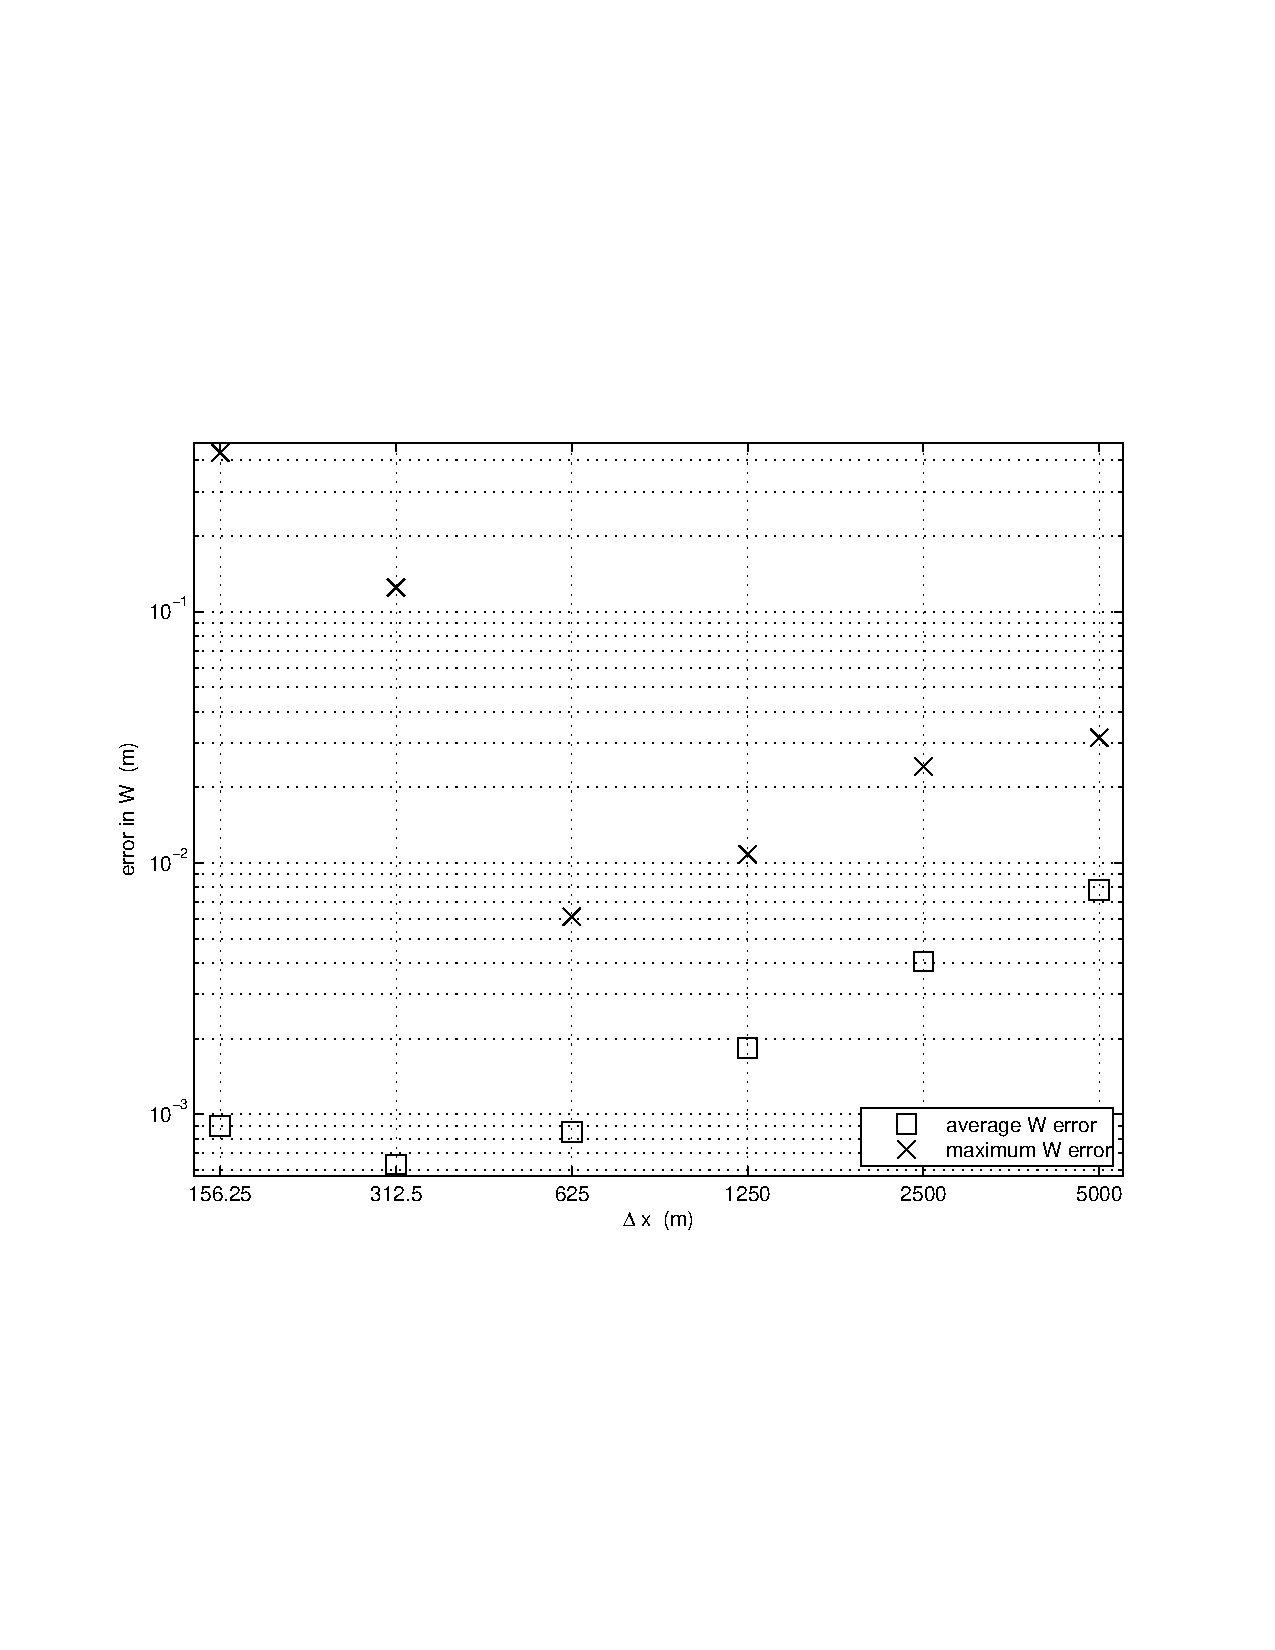
\includegraphics[width=3.0in,keepaspectratio=true]{refineWpism} \quad 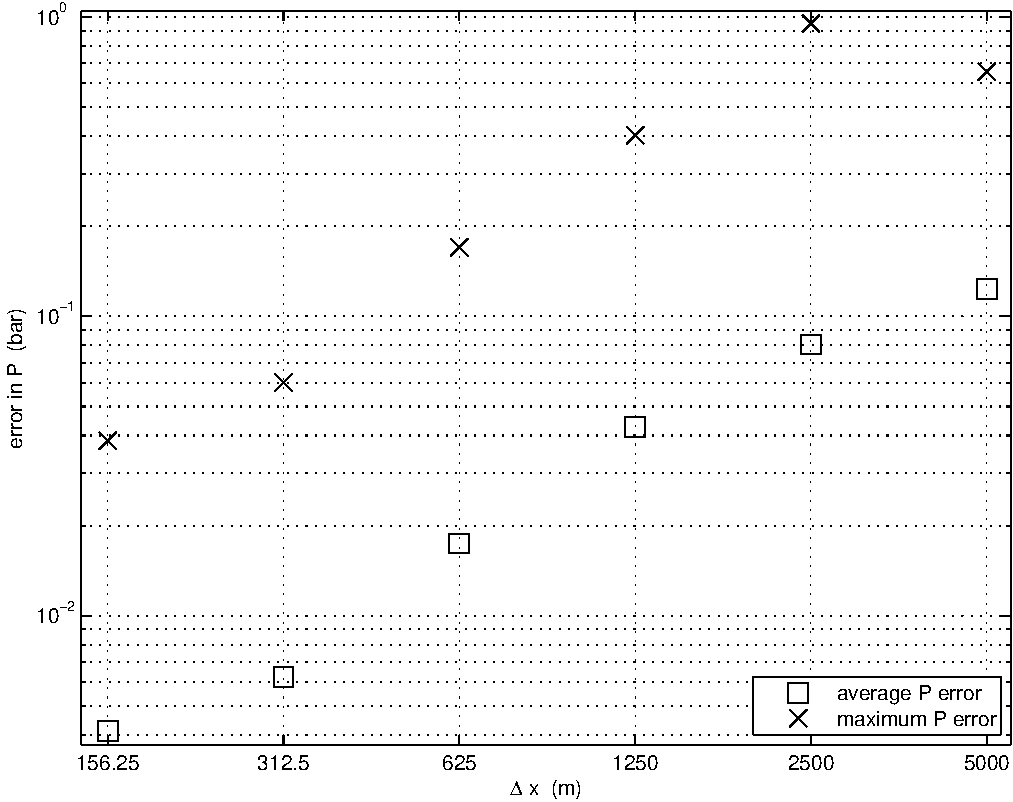
\includegraphics[width=3.0in,keepaspectratio=true]{refinePpism}
\caption{Left: Average water thickness error $|W-W_{exact}|$ decays as $O(\Delta x^{0.92})$ for $312.5 \le \Delta x \le 2500$ m.  Right: Average pressure error $|P-P_{exact}|$ decays as $O(\Delta x^{0.95})$ for the same grid-spacing range.}
\label{fig:refineWPpism}
\end{figure}

Because they give evidence for numerical convergence, these results suggest that our numerical solution method for these coupled advection-diffusion (for $W$) and diffusion-reaction (for $P$) equations are being solved correctly.  The rate of convergence is not very good, however.  The location of the large errors is entirely in the neighborhood of the ice margin $r=L$ (not shown).  The method for handling boundary conditions is therefore critical to reducing the magnitude of the error and increasing its rate of decay.  Further research is needed to decide how to handle this boundary in a more-nearly optimal manner.

The rates of convergence for average errors are nearly identical for the higher resolution flux-limited (Koren) scheme and for the first-order upwinding scheme (not shown).  Because our problem is an advection-diffusion problem in which both the advection velocity and the diffusivity are solution-dependent, it is difficult to separate the errors arising from the numerical treatments of advection and diffusion.  The first-order upwinding scheme for the advection has much larger numerical diffusivity but this diffusivity may be masked by the continuum model (i.e.~desirable) diffusivity.  Based on this verification evidence it is reasonable to choose first-order upwinding for applications.  This scheme is simpler to implement, requires fewer floating point operations, and requires less communication in a parallel implementation.



\section{Results}  \label{sec:results}

\subsection*{Steady results for a tidewater glacier}

FIXME: decide on where this paper is going

FIXME: redo results from nbreen to use PISM and make better figures


\begin{comment}
\begin{figure}[ht]
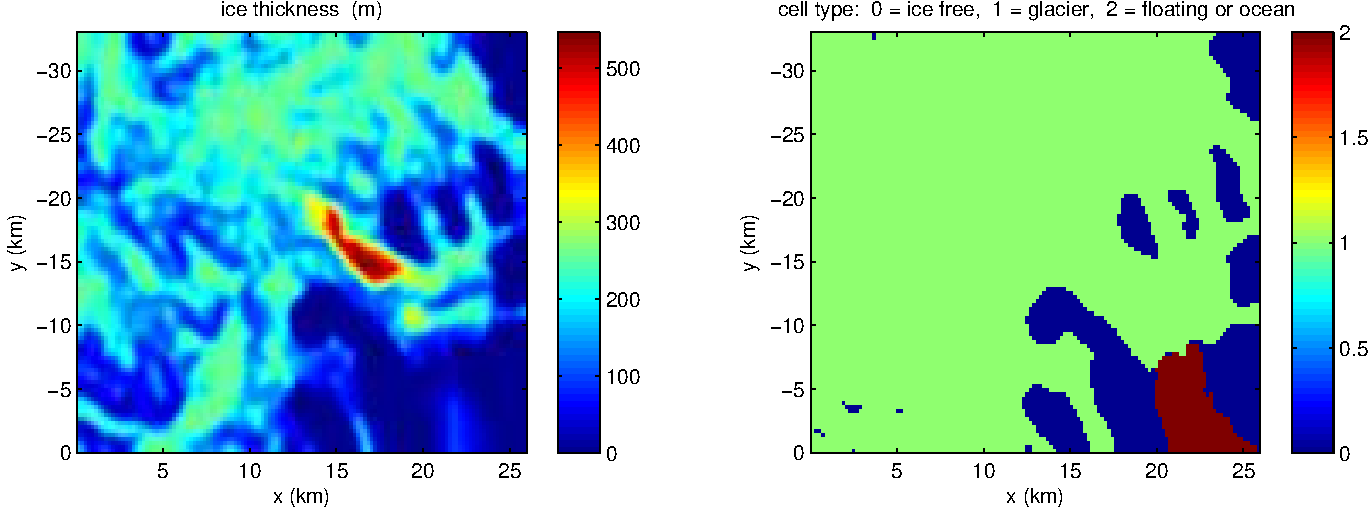
\includegraphics[width=7.0in,keepaspectratio=true]{icethk-icefree-float-250m}
\caption{FIXME}
%\label{fig:X}
\end{figure}

\begin{figure}[ht]
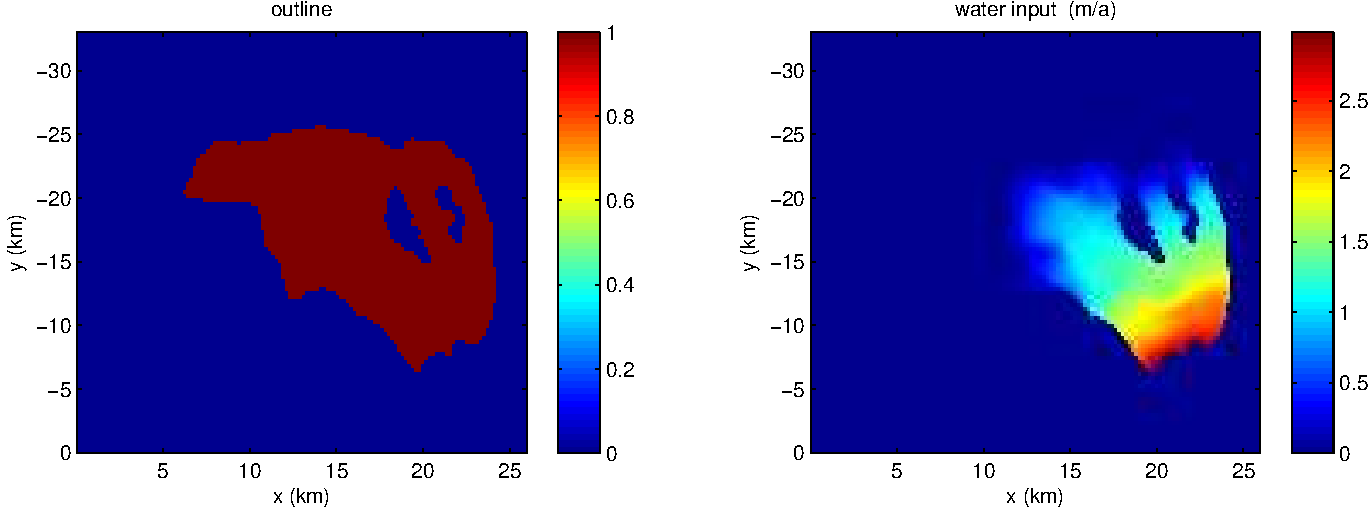
\includegraphics[width=7.0in,keepaspectratio=true]{outline-input-250m}
\caption{FIXME}
%\label{fig:X}
\end{figure}

\begin{figure}[ht]
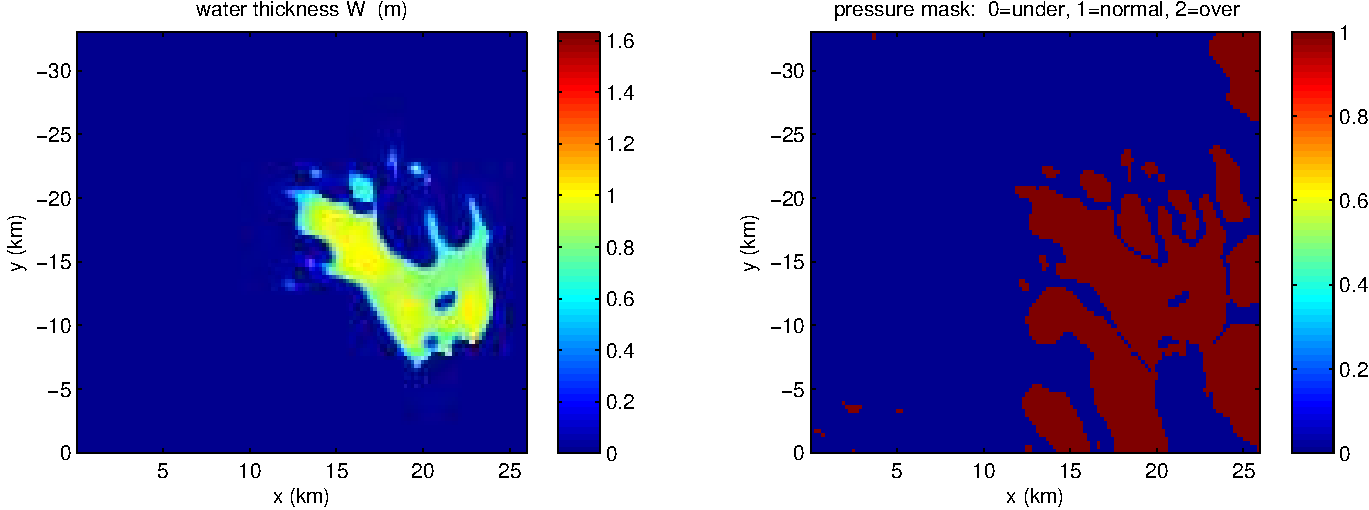
\includegraphics[width=7.0in,keepaspectratio=true]{W-Pmask-250m}
\caption{FIXME}
%\label{fig:X}
\end{figure}

\begin{figure}[ht]
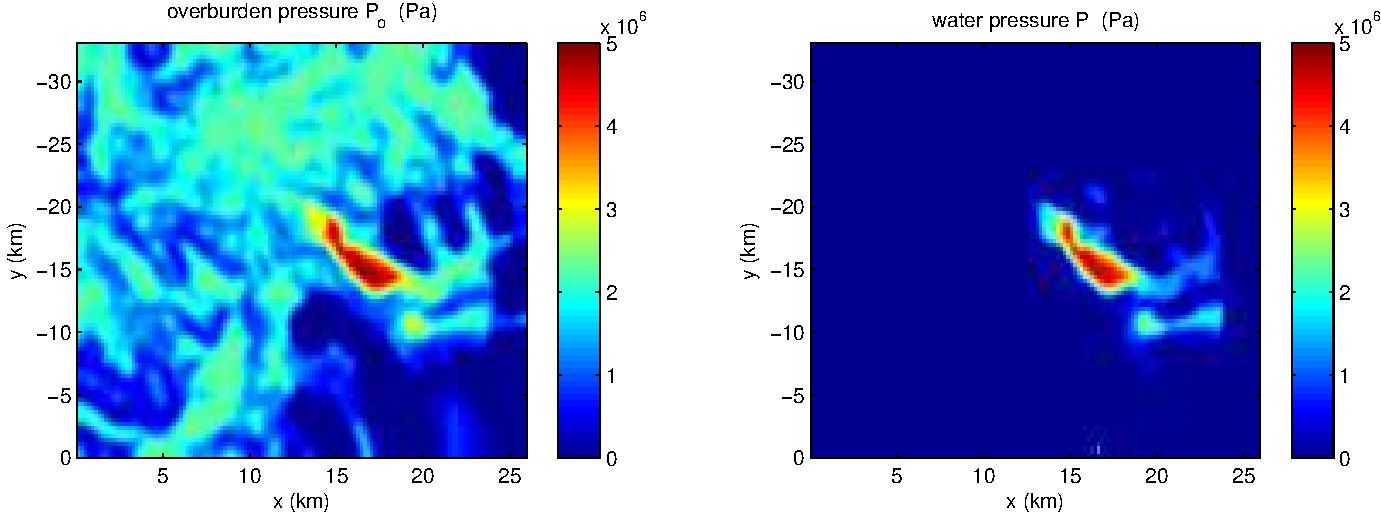
\includegraphics[width=7.0in,keepaspectratio=true]{Po-P-250m}
\caption{FIXME}
%\label{fig:X}
\end{figure}
\end{comment}

FIXME:  text about F\&C equation \eqref{eq:PofWFC}

\begin{figure}[ht]
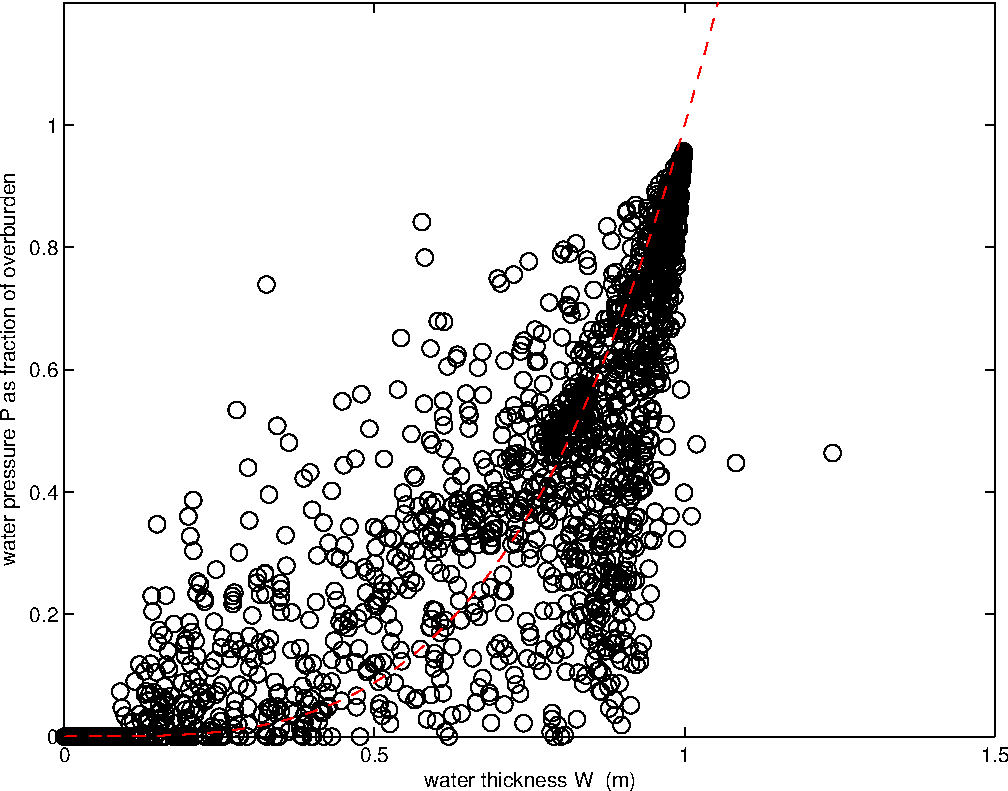
\includegraphics[width=3.0in,keepaspectratio=true]{isPofW-250m} \,
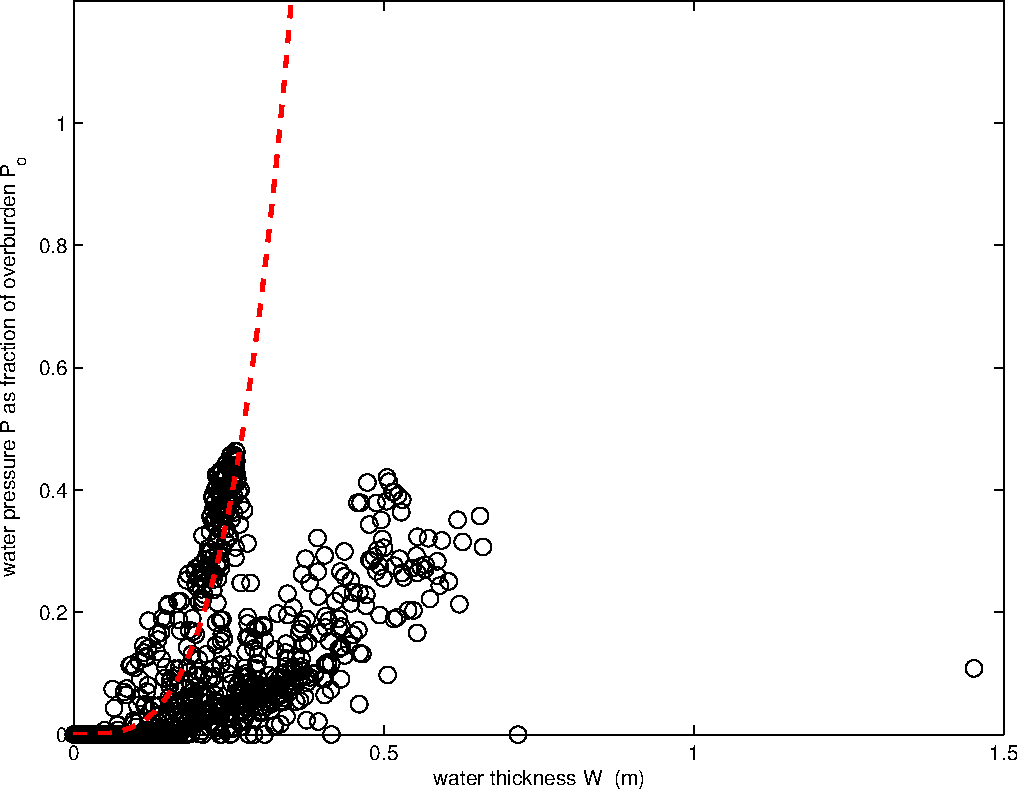
\includegraphics[width=3.0in,keepaspectratio=true]{isPofW-250m-month}
\caption{Left: Scatter plot of $(W,P)$ pairs for all cells at end of 5 year steady-input simulation on a 250 m grid.  Red dashed is equation \eqref{eq:PofWFC} with $W_{\text{crit}} = W_r = 1$ m.  Right: Same except at the end of a one month simulation, and with equation \eqref{eq:PofWFC} using $W_{\text{crit}} = W_r / 3$.}
\label{fig:isPofWnbreen}
\end{figure}


\section{Conclusion}  \label{sec:conclusion}

FIXME:  MOST IMPORTANT?:  IMPLEMENTED COMMON EXTENSION OF MAJOR MODELS


%\clearpage\newpage
\small
\bibliography{ice_bib}  % generally requires link to pism/doc/ice_bib.bib
\bibliographystyle{agu}
\normalsize


%\clearpage\newpage
\appendix
\small

\section{Relation to the Bartholomaus et al.~(2011) model}  \label{app:barth}

The model in \cite{Bartholomausetal2011} describes the evolution of the hydrology of the Kennicott glacier in Alaska.  It is a significantly different model from the distributed one of \cite{Schoofetal2012}, which we compare to in the main text, but similarities exist.  Both models describe the evolution of linked-cavity systems, and both include physical cavity opening and closing processes.  On the other hand the \cite{Schoofetal2012} theory is distributed and entirely subglacial while the \cite{Bartholomausetal2011} is ``lumped'' (i.e.~the entire glacier is represented by one cell) and is both subglacial and englacial.

In this Appendix we restate the published equations of the \cite{Bartholomausetal2011} model and then we derive a pressure evolution equation which applies in that model.  The form of this pressure equation is suggested by equation (12) in \cite{Bartholomausetal2011}, but its complete form is not stated.  By extending it to the distributed case, this pressure equation can be recognized as a diffusive (parabolic) version of the elliptic pressure equation in \cite{Schoofetal2012}.  This is one method for deriving our pressure equation \eqref{eq:regpressureequation} in the main text.

We start by describing the variables and equations of the \cite{Bartholomausetal2011} model.  The total volume of liquid water stored in the glacier is $S(t)$.  This is split into englacial $S_{en}(t)$ and subglacial $S_{sub}(t)$ portions.  The cavities have geometry partially-determined by bedrock bumps which have cartesian spacing $\lambda_x,\lambda_y$, height $h$, and width $w_c$.  These combine to give a dimensionless capacity parameter $f=(h w_c)/(\lambda_x \lambda_y)$; the value $f=0.05$ is used for the Kennicott glacier application.  Each cavity has cross-sectional area $A_c(t)$ and volume $w_c A_c$.  The glacier occupies a rectangle of dimensions $L\times W$ in the map-plane so that the number of cavities is $\nu = (LW)/(\lambda_x\lambda_y)$.  It follows that the subglacial storage volume is $S_{sub} = (w_c A_c) \nu = (f L W/h) A_c$.

Englacial water is assumed to fill crevasses and moulins up to a level $z_w(t)$ above the bedrock, in a system which has macroporosity $\phi$ (dimensionless).  Thus the englacial storage is $S_{en}=L W \phi z_w$.  In summary, the \cite{Bartholomausetal2011} model includes these equations describing the water amount variables $S_{en}$ and $S_{sub}$:
\begin{equation}
S = S_{en} + S_{sub}, \qquad S_{en} = L W \phi \zen, \qquad S_{sub} = \frac{f L W}{h} A_c.  \label{eq:barth:kinematics}
\end{equation}

Mass conservation in the model is the simple statement  \citep{Bartholomausetal2008}
\begin{equation}
\frac{dS}{dt} = Q_{in}(t) - Q_{out}(t). \label{eq:barth:massconserve}
\end{equation}
In the Kennicott glacier application, fluxes $Q_{in}$ and $Q_{out}$ are given by observations.

Let $P_o=\rho_i g H$ denote the overburden pressure, $P(t)$ the water pressure, and $N(t)=P_o-P(t)$ the effective pressure applied by the glacier to its bed.  Knowledge of the water pressure $P$ is equivalent to knowledge of the amount of englacial storage because there is an assumed efficient connection of the macroporous glacier to the subglacial system, namely the equation $S_{en}=L W \phi \zen$.  Englacial water therefore applies the hydrostatic pressure to the subglacier, and thus also
\begin{equation}
P = \rho_w g z_w.  \label{eq:barth:englacialpressure}
\end{equation}

In the \cite{Bartholomausetal2011} model the cavity cross-sectional area $A_c$ evolves by physical opening and closure processes.  A wall melt parameterization is also given but, in keeping with the cavity evolution in the rest of the current paper, we simply denote it as a melt term $\dot m$.  Denote the sliding speed by $u_b$ and let $C_c = (2 A)/n^n$, where $A$ and $n$ are parameters in the (Glen) ice flow law \citep{CuffeyPaterson}.  Then the cavity area evolution equation (4) in \cite{Bartholomausetal2011} is
\begin{equation}
\frac{dA_c}{dt} = \dot m + u_b h - C_c A_c (P_o-P)^n.  \label{eq:barth:cavityevolution}
\end{equation}
The three terms on the right are opening by cavitation, melt, and closure by creep, respectively.

Equations \eqref{eq:barth:kinematics}, \eqref{eq:barth:massconserve}, \eqref{eq:barth:englacialpressure}, and \eqref{eq:barth:cavityevolution} combine to give an evolution equation for the pressure, though this may not have been recognized by \cite{Bartholomausetal2011}.  From \eqref{eq:barth:kinematics} and \eqref{eq:barth:englacialpressure} we can write the pressure rate of change in terms of the englacial storage rate of change:
	$$\frac{dP}{dt} = \rho_w g \frac{dz_w}{dt} = \frac{\rho_w g}{L W \phi} \frac{d S_{en}}{dt}.$$
But \eqref{eq:barth:kinematics} and \eqref{eq:barth:massconserve}  allow us to rewrite in terms of fluxes and cavity area:
    $$\frac{dP}{dt} = \frac{\rho_w g}{L W \phi} \left(\frac{d S}{dt} - \frac{d S_{sub}}{dt}\right) = \frac{\rho_w g}{L W \phi} \left(Q_{in} - Q_{out} - \frac{d S_{sub}}{dt}\right).$$
Now use \eqref{eq:barth:kinematics} to write the evolution in terms of the rate of change of $A_c$:
    $$\frac{dP}{dt} = \frac{\rho_w g}{L W \phi} \left(Q_{in} - Q_{out} - \frac{f L }{h} \frac{d A_c}{dt}\right).$$
Finally incorporate equation \eqref{eq:barth:cavityevolution} to eliminate $dA_c/dt$:
\begin{equation}
\frac{dP}{dt} = \frac{\rho_w g}{L W \phi} \left(Q_{in} - Q_{out} - \frac{f L }{h} \left[\dot m + u_b h - C_c A_c (P_o-P)^n\right]\right)  \label{eq:barth:fullpressure}
\end{equation}
We emphasize that, though it is not stated there, equation \eqref{eq:barth:fullpressure} follows from the model equations in \cite{Bartholomausetal2011}.

Equation \eqref{eq:barth:fullpressure} suggests how to extend the \cite{Bartholomausetal2011} theory from ``lumped'' into ``distributed.''  Consider a one-dimensional glacier flowing in the positive $x$ direction.  Let the transverse width be $W$ and replace $L$ by $\Delta x$.  Note that ``$Q_{in}$'' would, in a distributed theory, be the upstream flux while ``$Q_{out}$'' would be downstream.  Thus we rewrite \eqref{eq:barth:fullpressure} as
\begin{equation*}
\frac{\phi}{\rho_w g}\frac{dP}{dt} = \frac{1}{W} \left(- \frac{Q_{out} - Q_{in}}{\Delta x} - \frac{f}{h} \left[\dot m + u_b h - C_c A_c (P_o-P)^n\right]\right).
\end{equation*}
The continuum limit is then clear, with $(Q_{out} - Q_{in})/\Delta x \to \partial Q/\partial x$.  Thus a distributed flowline form of the \cite{Bartholomausetal2011} theory is the partial differential equation
\begin{equation}
\frac{\phi}{\rho_w g} \frac{\partial P}{\partial t} = \frac{1}{W} \left(- \frac{\partial Q}{\partial x} - \frac{f}{h} \left[\dot m + u_b h - C_c A_c (P_o-P)^n\right]\right).  \label{eq:barth:distpressure}
\end{equation}
Equation \eqref{eq:barth:distpressure} is, for all practical purposes, the same as equation \eqref{eq:regpressureequation} in the main text.

A distributed extension of the \cite{Bartholomausetal2011} theory is not, however, viable without a Darcy or other flux expression for $Q$.  One must also use a distributed mass conservation equation like \eqref{eq:conserve}.  By contrast, a flux expression, Darcy or otherwise, was not needed in the Kennicott glacier case because the lumped input and output from the hydrological system were available as data.

An implication of the \cite{Bartholomausetal2011} model, again not stated there, regards the pressure in steady state.  Steady state in equation \eqref{eq:barth:cavityevolution} gives
\begin{equation*}
0 = \dot m + u_b h - C_c A_c (P_o-P)^n.
\end{equation*}
This is a relationship between pressure $P$ and cavity area $A_c$ in steady state:
\begin{equation}
P = P_o - \left(\frac{\dot m + u_b h}{C_c A_c}\right)^{1/n}. \label{eq:barth:steadypressure}
\end{equation}
This equation, which is just like equation \eqref{eq:PofWsteady} in the main text, says that in steady state the pressure is a function of the amount of water.  It is interesting to observe, however, that \eqref{eq:barth:steadypressure} shows that the steady water pressure does not depend on the englacial macroporosity $\phi$.  Though the englacial pressure is parameterized by $P=\rho_w g z_w$ in \cite{Bartholomausetal2011}, its \emph{steady} value is entirely determined by the balance between sliding, wall melt, and creep closure in the subglacial system.  The englacial system is passive in determining steady state.

Returning to equation \eqref{eq:barth:distpressure} we can now connect the theory outlined in this Appendix with the main theory in the paper.  Namely, if we extend \eqref{eq:barth:distpressure} to two horizontal dimensions ($\partial Q/\partial t \to \Div \bq$ and so on) and we add Darcy relation \eqref{eq:flux} then we get \eqref{eq:regpressureequation}.  Under any reasonable Darcy-type formulation for the flux $Q$ in \eqref{eq:barth:distpressure}, the $\phi\to 0$ limit of \eqref{eq:barth:distpressure} is an elliptic equation for the water pressure.  This $\phi\to 0$ limit of the distributed version of the \cite{Bartholomausetal2011} model is the model in \cite{Schoofetal2012}.  The main text of the current paper simultaneously describes a distributed extension of the \cite{Bartholomausetal2011} model and an englacial-storage-regularized extension of the \cite{Schoofetal2012} model.


\section{An abstract view of the transport-plus-storage problem} \label{app:transportstorage}

The problem considered in sections \ref{sec:elements} and \ref{sec:capacity} includes a mass conservation equation for the total water amount, a portion of which is transportable, and an equation for the evolution of the water stored locally in till pore spaces.  In this Appendix we treat such a pair of coupled equations abstractly.  We show some mathematical properties of the continuum equations, and we show important properties of a simple numerical scheme for these equations.

The abstract view in this Appendix starts by stating a pair of abstract equations for abstract quantities $u(t,x,y),v(t,x,y)$ satisfying bounds $u\ge 0$ and $0 \le v \le v_{\text{max}}$:
\begin{align}
\frac{\partial}{\partial t} \left(u+v\right) &= \Div \bq + g, \label{eq:abs:transport} \\
   \frac{\partial v}{\partial t} &= b \left(f - v\right).  \label{eq:abs:storage}
\end{align}
Here the conserved quantity is the sum $u+v$.  The flux $\bq(x,y,u,\grad u)$ depends on the transported portion $u$, and its gradient, but not on the locally-stored portion $v$.  The source term can depend on location: $g(x,y)$.  The term $f(x,y,u)$ could be called the ``transfer target''; like $v$ it satisfies bounds $0 \le f \le v_{\text{max}}$.

To relate this to the main text, $u$ is analogous to the transportable water $W$ and $v$ to the till-stored water $\Wtil$.  Equation \eqref{eq:abs:transport} is an abstract form of the original mass-conservation equation \eqref{eq:conserve}, while \eqref{eq:abs:storage} is the abstract form of \eqref{eq:tilldynamics}.

Equation \eqref{eq:abs:transport} says that the sum $u+v$ is conserved as it evolves by transport and creation/removal.  Equation \eqref{eq:abs:storage} describes local (i.e.~with no spatial derivatives) evolution of the locally-stored quantity $v$.  The flux $\bq$ and the source term $g$ in \eqref{eq:abs:transport} are quite general, and the details generally don't concern us here.  Also, the details of the transfer target $f$ are unimportant.  The constant $b\ge 0$ in \eqref{eq:abs:storage} is the exponential rate at which the locally-stored quantity would ``drain'' in the absence of transfer of $u$, in the sense that $v(t) = v_0 e^{-bt}$ is the solution of \eqref{eq:abs:storage} if $f=0$.

We now demonstrate properties of this abstract structure:

\renewcommand{\labelenumi}{\arabic{enumi}.\quad}

\begin{enumerate}
\item  \emph{Alternative integration-over-history interpretation.}  The storage quantity $v$ could be eliminated from the system of equations \eqref{eq:abs:transport} and \eqref{eq:abs:storage}.  The result is a single transport equation for $u$ which has a term which is an integral over previous states of $u$.  Implementing this equation is impractical; it would require storage of prior states.  However, we go ahead and show how to eliminate $v$ so as to understand the equations better.  

Multiply \eqref{eq:abs:storage} by an integrating factor $e^{-bt}$ and simplify to get the form $\partial_t (e^{bt} v) = b e^{bt} f$.  If $v$ is known at the initial time, say $v=v_0(x,y)$ at $t=0$, then we can integrate from $0$ to $t$ and multiply both sides by $e^{-bt}$ to get
\begin{equation}
v(t,x,y) = e^{-bt} \left(v_0(x,y) + b \int_0^t e^{bs} f(x,y,u(s,x,y))\,ds\right). \label{eq:abs:vexpression}
\end{equation}
This allows us to eliminate $v$ from \eqref{eq:abs:transport} by moving $\partial v/\partial t$ to the right side:
\begin{equation}
\frac{\partial u}{\partial t} = \Div \left(\mathbf{q}\right) + g + b e^{-bt} v_0 - b f + b^2 \int_0^t e^{-b(t-s)} f\,ds. \label{eq:abs:historyintegration} 
\end{equation}
Thus we can eliminate the locally-stored quantity $v$ at the cost of maintaining a complete history of the past values of the transported quantity $u$, so as to be able to compute the integral on the right in \eqref{eq:abs:historyintegration}.  While equation \eqref{eq:abs:historyintegration} may be conceptually advantageous, because it has only one conserved scalar $u$, it is not effectively-implementable.
\medskip

\item \emph{An implicit scheme for \eqref{eq:abs:storage}, and its properties.}  Equation \eqref{eq:abs:storage} is linear in $v$ and it has no spatial derivatives, so we can easily implement an implicit numerical scheme which has no stability restrictions on time steps, and for which we can prove desirable inequalities.  The backwards Euler approximation of \eqref{eq:abs:storage} is stable (``A-stable'' \citep{AscherPetzold}); we state two equivalent forms:
\begin{equation}
\frac{V^{l+1} - V^l}{\Delta t} = b \left(f^l - V^{l+1}\right) \qquad \iff \qquad
V^{l+1} = \frac{V^l + b \Delta t f^l}{1 + b \Delta t}.  \label{eq:abs:Vupdate}
\end{equation}
(Compare equation \eqref{eq:tillupdatefd}.)

Noting $b \Delta t \ge 0$ we see that $V^{l+1}$ in \eqref{eq:abs:Vupdate} is an \emph{average} of $V^l$ and $f^l$.  Therefore
\begin{equation}
0 \le V^l, f^l \le v_{\text{max}} \quad \implies \quad 0 \le V^{l+1} \le v_{\text{max}}. \label{eq:abs:Vbounds}
\end{equation}
Thus the discrete evolution of the locally-stored quantity $v$ maintains the needed bounds.  It is also easy to prove that if the transfer target term $f$ is constant in time, e.g.~if $f^{l-1}=f^1=\tilde f$ in \eqref{eq:abs:Vupdate}, then the local storage quantity $V^l$ strictly approaches the transfer target on consecutive time steps, that is,
\begin{equation}
\left|V^{l+1} - \tilde f\right| < \left|V^l - \tilde f\right|, \label{eq:abs:Vapproach}
\end{equation}
assuming $b\Delta t > 0$.  Properties \eqref{eq:abs:Vbounds} and \eqref{eq:abs:Vupdate} would have to be separately enforced in an explicit scheme.
\medskip

\item \emph{Discretization of \eqref{eq:abs:transport}}.  We can fully-discretize equation \eqref{eq:abs:transport} using an mostly-explicit scheme with centered-difference approximation of the divergence of the flux, and using staggered-grid values of the flux.  In fact, let $t^{l+1}-t^l = \Delta t$ be the time step and suppose $U^l,V^l$ approximate $u,v$ at time $t^l$.  If we denote $\bq = (q^x,q^y)$ then we can write the scheme as
\begin{align}
\frac{U_{i,j}^{l+1} - U_{i,j}^l}{\Delta t} &= \frac{q^x_{i+1/2,j} - q^x_{i-1/2,j}}{\Delta x} + \frac{q^y_{i,j+1/2} - q^y_{i,j-1/2}}{\Delta y} + g_{ij} - \frac{V_{i,j}^{l+1} - V_{i,j}^l}{\Delta t}. \label{eq:abs:conservefd}
\end{align}

The goal is to update $U$ to time $t^{l+1}$.  Scheme \eqref{eq:abs:conservefd} supposes values $\{U_{ij}^l,V_{ij}^l\}$ are available.  But we use \eqref{eq:abs:conservefd} \emph{after} we use \eqref{eq:abs:Vupdate} because \eqref{eq:abs:conservefd} also requires $ V_{i,j}^{l+1}$.  The staggered-grid flux components in \eqref{eq:abs:conservefd} must be computed in some manner from the various known values, but the details are unimportant here.  Stability and positivity of scheme \eqref{eq:abs:conservefd} is addressed in Appendix \ref{app:positivestable}.  Stability depends on how fluxes are evaluated; see Appendix \ref{app:fluxlimiters}.
\medskip

\item \emph{Discrete conservation}.  We can prove that equations \eqref{eq:abs:Vupdate} and \eqref{eq:abs:conservefd} conserve the discrete version of the sum $u+v$.  The continuum conservation statement, which follows from \eqref{eq:abs:transport} by using the divergence theorem, is, on a region $R$ of the $x,y$ plane,
\begin{equation}
\frac{d}{dt} \left(\int_R u + v\,dx dy\right) = \int_{\partial R} \bq \cdot \bn\,ds + \int_R g \,dx dy.  \label{eq:abs:continuumconserve}
\end{equation}

One may think in finite volume terms of the regular grid quantities $U_{ij}^l,V_{ij}^l$ as being the average values over cells.  The integrals over $R$ in \eqref{eq:abs:continuumconserve} are then approximated by the midpoint integration rule.  Specifically, the discrete analogue of the integral over $R$ of $u+v$ is this discrete total volume sum in the case where $R$ is a rectangle:
\begin{equation}
\Theta^l = \sum_{i,j=1,1}^{I,J} \left(U_{ij}^l + V_{ij}^l\right)\,\Delta x \Delta y \approx 
\int_R u(t^l,x,y) + v(t^l,x,y) \,dx dy\end{equation}

Discrete conservation of $\Theta^l$ is exact even though $\Theta^l$ only approximates the continuum value of the total volume:
\begin{align}
\frac{\Theta^{l+1} - \Theta^l}{\Delta t} &= \sum_{i,j} \frac{U_{ij}^{l+1} - U_{ij}^l}{\Delta t} \,\Delta x \Delta y   + \sum_{i,j} \frac{V_{ij}^{l+1} - V_{ij}^l}{\Delta t} \,\Delta x \Delta y   \label{eq:abs:discreteconserve} \\
  &\stackrel{\ast}{=} \sum_{i,j} \left(\frac{q^x_{i+1/2,j} - q^x_{i-1/2,j}}{\Delta x} + \frac{q^y_{i,j+1/2} - q^y_{i,j-1/2}}{\Delta y} + g_{ij} - \frac{V_{i,j}^{l+1} - V_{i,j}^l}{\Delta t}\right) \,\Delta x \Delta y  \notag \\
  &\qquad\qquad + \sum_{i,j} \frac{V_{ij}^{l+1} - V_{ij}^l}{\Delta t} \,\Delta x \Delta y   \notag \\
  &= \sum_{j=1}^{J} \left(\sum_{i=1}^{I}  q^x_{i+1/2,j} - q^x_{i-1/2,j}\right) \Delta y +  \sum_{i=1}^{I} \left(\sum_{j=1}^{J} q^y_{i,j+1/2} - q^y_{i,j-1/2}\right) \Delta x +  \sum_{i,j} g_{ij}\,\Delta x \Delta y  \notag \\
  &\stackrel{\dagger}{=} \sum_{j=1}^{J} \left(q^x_{I+1/2,j} - q^x_{1/2,j}\right) \Delta y +  \sum_{i=1}^{I} \left(q^y_{i,J+1/2} - q^y_{i,1/2}\right) \Delta x +  \sum_{i,j} g_{ij}\,\Delta x \Delta y \notag \\
  &= \left[- \sum_{i=1}^{I}  q^y_{i,1/2} \Delta x + \sum_{j=1}^{J} q^x_{I+1/2,j} \Delta y + \sum_{i=1}^{I} q^y_{i,J+1/2} \Delta x - \sum_{j=1}^{J} q^x_{1/2,j} \Delta y \right]  +  \sum_{i,j} g_{ij}\,\Delta x \Delta y. \notag
\end{align}
Step $\ast$ follows from \eqref{eq:abs:conservefd}.  Step $\dagger$ follows from noticing that the inside sums collapse though cancellation.  The four sums inside square brackets in the last line are sums over consecutive sides of the rectangle $R$, starting in the lower-left and traversing counterclockwise.

Our statement \eqref{eq:abs:discreteconserve} of discrete conservation should now be compared  to the continuum statement \eqref{eq:abs:continuumconserve}.
\end{enumerate}


\section{Positivity and stability of the mass conservation scheme} \label{app:positivestable}

Explicit numerical scheme \eqref{eq:Wupdate} for the mass conservation PDE \eqref{eq:adeqn}, combined with the first-order upwind case of formulas \eqref{eq:adfluxes}, is sufficiently simple so that we can analyze its stability properties.  For this scheme we sketch a maximum principle argument which shows stability \citep{MortonMayers}.  The argument also shows positivity \citep{HundsdorferVerwer2010} as long as the total water input is nonnegative; here only the case $m = 0$ is shown.  We consider only the upwinding case where the discrete velocities at cell interfaces are nonnegative: $u_e\ge 0$, $u_w\ge 0$, $v_n\ge 0$, $v_s\ge 0$.  The other upwinding cases can be handled by similar special-case arguments like this one.

We start by restating equation \eqref{eq:Wupdate} with the above simplifications, also defining $\nu_x = \Delta t/\Delta x$, $\nu_y = \Delta t/\Delta y$, $\mu_x = \Delta t/\Delta x^2$, and $\mu_y = \Delta t/\Delta y^2$:
\begin{align*}
 W_{i,j}^{l+1} &= \Wlij - \nu_x \left(u_e \Wlij - u_w W_{i-1,j}^l\right) - \nu_y \left(v_n \Wlij - v_s W_{i,j-1}^l\right)  \\
      &\qquad + \mu_x \left[D_e \left(W_{i+1,j}^l - \Wlij\right) - D_w \left(\Wlij - W_{i-1,j}^l\right)\right]  \\
      &\qquad + \mu_y \left[D_n \left(W_{i,j+1}^l - \Wlij\right) - D_s \left(\Wlij - W_{i,j-1}^l\right)\right].
\end{align*}
Collecting terms to write the new value as a linear combination of the old values, we get
\begin{align}
 W_{i,j}^{l+1} &= (\nu_x u_w + \mu_x D_w) W_{i-1,j}^l + (\mu_x D_e) W_{i+1,j}^l + (\nu_y v_s + \mu_y D_s) W_{i,j-1}^l + (\mu_y D_n) W_{i,j+1}^l  \notag \\
      &\qquad + \Big[1 - \nu_x u_e - \nu_y v_n - \mu_x (D_e + D_w) - \mu_y (D_n + D_s)\Big] \Wlij \notag \\
  &= \tilde A\, W_{i-1,j}^l + \tilde B\, W_{i+1,j}^l + \tilde C\, W_{i,j-1}^l + \tilde D\, W_{i,j+1}^l + \tilde E\, \Wlij. \label{eq:lincomb}
\end{align}
Because of our assumption about nonnegative velocities, and noting that the diffusivities are nonnegative, we see that coefficients $\tilde A,\tilde B,\tilde C,\tilde D$ are all nonnegative.  Only $\tilde E$ could be negative, depending on values of $\nu_x, \nu_y, \mu_x$, and $\mu_y$.  Requiring it to be nonnegative will generate a sufficient stability condition \citep{MortonMayers}.

We state such a condition based on an equal split between advective and diffusive parts.  First there is a CFL restriction for the advection terms; compare \eqref{eq:dtCFL}:
\begin{equation}
\nu_x \alpha_e + \nu_y \beta_n = \Delta t \left(\frac{u_e}{\Delta x} + \frac{u_n}{\Delta y}\right) \le \frac{1}{2}. \label{eq:adstabcond}
\end{equation}
The second is a time-step restriction on the diffusion; compare \eqref{eq:dtDIFFW}:
\begin{equation}
\mu_x (D_e + D_w) + \mu_y (D_n + D_s) = \Delta t \left(\frac{D_e + D_w}{\Delta x^2} + \frac{D_n + D_s}{\Delta y^2}\right) \le \frac{1}{2}. \label{eq:diffstabcond}
\end{equation}
If \eqref{eq:adstabcond} and \eqref{eq:diffstabcond} hold then the coefficient $\tilde E$ in \eqref{eq:lincomb} is nonnegative:
	$$\tilde E = 1 - \nu_x u_e - \nu_y v_n - \mu_x (D_e + D_w) - \mu_y (D_n + D_s) \ge 0.$$

Because the coefficients in linear combination \eqref{eq:lincomb} add to one, as the reader may check, it follows  from \eqref{eq:adstabcond} and \eqref{eq:diffstabcond} that the scheme is stable \citep{MortonMayers}.  It also follows from \eqref{eq:adstabcond} and \eqref{eq:diffstabcond} that if $\Wlij\ge 0$ for all $i,j$ then \eqref{eq:lincomb} gives $W_{ij}^{l+1}\ge 0$, which is our positivity claim.  More generally, under conditions \eqref{eq:dtCFL} and \eqref{eq:dtDIFFW}, the conditions which describe all of the upwinding cases, scheme \eqref{eq:Wupdate} is stable and positivity-preserving.


\section{Flux-limiter methods} \label{app:fluxlimiters}

Because \eqref{eq:adeqn} in the main text is an advection-dominated PDE, the well-known goals for discretizing the fluxes in \eqref{eq:adeqn} include non-oscillation and positivity \citep{HundsdorferVerwer2010} in addition to reduced truncation error.  Schemes addressing these goals are often described as finite volume discretizations \citep{LeVeque}.  We now introduce a few such schemes using an advection-only model equation in which an abstract quantity $u(t,x)$ is transported by an abstract velocity $v(x)$:
\begin{equation} \label{eq:modeladvect}
\ddt{u} + \ddx{}\left(v(x) u\right) = 0
\end{equation}

Suppose that the grid points $x_i$ are the centers of equally-spaced cells with $x_{i+1}-x_i=\Delta x$.  Cell interfaces are at $x_{i-1/2}=x_w$ (``\emph{w}'' for ``west'') and $x_{i+1/2}=x_e$ (``east'').  Suppose we do not discretize time and instead we denote $u(t,x_i)$ by $u_i(t)$.  We say a spatial discretization of \eqref{eq:modeladvect} is \emph{positive} if $u_i(0) \ge 0$ for all $i$ implies $u_i(t)\ge 0$ for all $t\ge 0$ and all $i$.  In particular, such a property is desirable for any conservation scheme for the water thickness because thicknesses are intrinsically nonnegative.

The discretizations of \eqref{eq:modeladvect} we consider here all use the fluxes $Q=v(x) u$ at the cell interfaces $x_w$ and $x_e$, namely
\begin{equation}
\frac{du_i}{dt} + \frac{Q_e - Q_w}{\Delta x} = 0. \label{eq:basicmodelFD}
\end{equation}
But we must choose a flux parameterization.  The simplest positive scheme for the fluxes is first-order upwinding in conservative form \citep[section I.4.3]{HundsdorferVerwer2010}.  We use the upwind value $u_i$ in $Q_e$ if $v_e = v(x_e) \ge 0$:
\begin{equation}
Q_e = v_e u_i \label{eq:upwindfluxfirst}
\end{equation}
If $v_e < 0$ then \eqref{eq:upwindfluxfirst} is replaced by $Q_e = v_e u_{i+1}$. 
Also $Q_w = v_w x_{i-1}$ if $v_w \ge 0$, and $Q_w = v_w x_{i}$ if $v_w < 0$.  Scheme \eqref{eq:upwindfluxfirst} is also called the ``donor cell'' upwind method \citep{LeVeque} because there is a decision, based on the sign of the cell-interface velocity, on which cell contributes the value of $u$.

A second-order truncation error scheme which is \emph{not} positive uses a centered average in computing the flux.  We can regard this as a correction to the first-order upwind form:
\begin{equation}
Q_e = v_e \frac{u_i+u_{i+1}}{2} = v_e \left[u_i + \frac{1}{2} (u_{i+1} - u_i)\right]. \label{eq:centerfluxfirst}
\end{equation}
A yet higher-resolution scheme is third-order upwind-biased fluxes which can again be written as a correction to first-order upwinding:
\begin{equation}
Q_e = v_e \frac{-u_{j-1} + 5 u_i + 2 u_{i+1}}{6} = v_e \left[u_i + \left(\frac{1}{3}+\frac{1}{6} \theta_i \right) (u_{i+1} - u_i)\right] \label{eq:thirdfluxfirst}
\end{equation}
where
\begin{equation}
\theta_i = \frac{u_{i} - u_{i-1}}{u_{i+1} - u_i}.  \label{eq:thetadefine}
\end{equation}
Unfortunately, despite the upwind-biasing in the third-order scheme, both \eqref{eq:centerfluxfirst} and \eqref{eq:thirdfluxfirst} cause oscillations and are not positive.

The ``flux-limiting'' (i.e.~flux-correction-limited) approach regards the corrections in \eqref{eq:centerfluxfirst} and \eqref{eq:thirdfluxfirst} as too large to allow positivity, specifically near local extrema of $u$ \citep[section III.1.1]{HundsdorferVerwer2010}.  Godunov's barrier theorem \citep[section I.7.1]{HundsdorferVerwer2010} says that we cannot get truncation error better than first-order with a discretization that is both linear and positive.  However, there exist nonlinear flux-limited formulas which restore these properties, and we list and try them here.  Because the schemes under consideration are explicit, the nonlinearity does not represent a significant computational cost.

These flux-limited schemes can be written in the same general form as above, with a correction to the first-order upwinded flux:
\begin{equation}
Q_e = v_e \left[u_i + \Psi(\theta_i) (u_{i+1} - u_i)\right], \qquad v_e \ge 0. \label{eq:fluxlimiterform}
\end{equation}
If we have $v(x)<0$ in \eqref{eq:modeladvect} then the same function $\Psi$ should be used but with the direction reversed \citep[section III.1.1]{HundsdorferVerwer2010}:
\begin{equation}
Q_e = v_e \left[u_{i+1} + \Psi\left((\theta_{i+1})^{-1}\right) (u_i - u_{i+1})\right], \qquad v_e < 0. \label{eq:fluxlimiterformreversed}
\end{equation}
The forms for $Q_w$ in \eqref{eq:basicmodelFD} simply replace $v_e \to v_w$, $i\to i-1$, and $i+1\to i$.  Table \ref{tab:fluxlimiters} shows several cases for $\Psi$ including those already considered.

The difference ratio $\theta_i$ in \eqref{eq:thetadefine} can take any real value.  For the time-discretizations we will consider, sufficient conditions on $\Psi(\theta)$ to give a positive advection scheme for model equation \eqref{eq:modeladvect} are
\begin{equation}
0 \le \Psi(\theta) \le 1, \qquad 0 \le \frac{\Psi(\theta)}{\theta} \le 1 \qquad \text{ for all } \theta \in \RR.
\end{equation}
The schemes in Table \ref{tab:fluxlimiters} which satisfy these conditions are marked with ``$\ast$''.

For smooth functions and fine grids we have $\theta_i\approx 1$ except near extrema where $u_{i+1} - u_i$ and $u_i - u_{i-1}$ are both near zero.  Note that in every case in Table \ref{tab:fluxlimiters} where there is a correction ($\Psi(\theta)\ne 0$) we have $\Psi(1)=1/2$.  The Koren flux-limiter in Table \ref{tab:fluxlimiters} \citep{HundsdorferVerwer2010} has $\Psi(\theta) = \frac{1}{3}+\frac{1}{6} \theta$ for $\frac{2}{5} \le \theta \le 4$.  We can think of the Koren scheme as a positive form of the third-order upwind-biased scheme.

\begin{table}[ht]
  \centering
  \caption{Flux schemes written in limiter form \eqref{eq:fluxlimiterform} using $\theta=\theta_i$ from \eqref{eq:thetadefine}. The formal ``order'' of the van Leer and Koren schemes only apply away from  ``difficult areas''; see text.}
  \begin{tabular}{lccl}
    \textbf{scheme} & \textbf{positive?} & \textbf{order} & \textbf{formula} \\
\hline
    simple upwinding & yes & 1 & $\phantom{\Big|}\Psi(\theta) = 0$ \\
    centered         & no  & 2 & $\phantom{\Big|}\Psi(\theta) = \frac{1}{2}$  \\
    upwind-biased    & no  & 3 & $\phantom{\Big|}\Psi(\theta) = \frac{1}{3}+\frac{1}{6} \theta$  \\
    van Leer 1974    & yes & 2 & $\phantom{\Big|}\Psi(\theta) = \frac{1}{2} \frac{\theta + |\theta|}{1+\theta}$  \\
    Koren 1993       & yes & 3 & $\phantom{\Big|}\Psi(\theta) = \max\left\{0,\min\{1,\theta,\frac{1}{3}+\frac{1}{6} \theta\}\right\}$  \\
    \hline
  \end{tabular}
 \label{tab:fluxlimiters}
\end{table}

To summarize the flux discretization choices for model equation \eqref{eq:modeladvect}, first-order upwinding \eqref{eq:upwindfluxfirst} gives positivity but only $O(\Delta x^1)$ truncation error while second-order centered differencing \eqref{eq:centerfluxfirst} and third-order upwind-biased differencing \eqref{eq:thirdfluxfirst} give better truncation error (i.e.~$O(\Delta x^2)$ and $O(\Delta x^3)$, respectively), but not positivity.  The flux-limited Koren and van Leer schemes in Table \ref{tab:fluxlimiters} give positivity and also better truncation error away from ``difficult areas''.  Such areas, which are where $\theta_i$ in \eqref{eq:thetadefine} is $\gg 1$ or $\ll 1$, tend to be near extrema and non-smooth areas.  Thus these schemes are high-order but they (nonlinearly) revert to first-order when they get in trouble.

The above discussion was limited to the spatial (semi-)discretization.  A time discretization is also required, and for this we simply choose forward Euler.  The fully discrete system is positive if
\begin{equation}
\max_x \frac{|v(x)|\Delta t}{\Delta x} \le \frac{1}{2} \label{eq:CFL}
\end{equation}
\citep[section III.1.1]{HundsdorferVerwer2010}.  One can show that these positive schemes are also total variation diminishing (TVD) if the velocity is constant ($v(x)=v_0$).  We identify condition \eqref{eq:CFL} as simply ``CFL'' even though it is more strict than the CFL condition that suffices for stability \citep{MortonMayers}.


\end{document}
